\documentclass[12pt]{UIdahoMastersThesis}
\makeatletter

%\includeonly{Chapters/Introduction}

\usepackage[latin1]{inputenc}
\usepackage{times}
\makenoidxglossaries

%Preamble
\usepackage{tikz,pgfplots,grffile}
\usetikzlibrary{positioning,plotmarks,arrows.meta}
\usetikzlibrary{calc,shapes.geometric}
\pgfplotsset{compat=newest}
\usepgfplotslibrary{patchplots}

\graphicspath{ {./img/} }

%\usepackage[PetersLenny]{fncychap} %This makes the chapter titles fancy: If you don't want it fancy, delete this line and the chapter title formatting under the \frontmatter below
	%\ChNameVar{\LARGE\scshape}
	%\ChTitleVar{\Huge\scshape}

%Make post-it notes!
\usepackage[colorinlistoftodos,prependcaption,textsize=tiny]{todonotes}
\newcommandx{\note}[2][1=]{\todo[linecolor=orange,backgroundcolor=yellow!25,bordercolor=orange,#1]{#2}}


\usepackage[capitalise,noabbrev]{cleveref}
% --------------------------------------------------------------------------
% Thesis Information
\title{Dynamic System Modeling \& \acs{pid} Controller Design \\for a Molten Salt Microreactor}
\author{Sam J. Root}
\thesisdegree{Master of Science}
\major{Nuclear Engineering}
\advisor{Michael G. McKellar, Ph.D.}
\cmone{Dakota Roberson, Ph.D.}
\cmtwo{Robert A. Borrelli, Ph.D.}
\deptadmin{Indrajit Charit, Ph.D.}
\graddate{December 2023}
% -------------------------------------------------------------------------

\linespread{1.3}%1.3 is on-and-a-half-spacing

% Defines section counter for front-matter. This way section number does not appear in the TOC for front-matter sections
\setcounter{secnumdepth}{0}

% Sets what level of sections show up in the table of contents. 0 = sections, 1 = subsections, 2 = sub-subsections, etc.
\setcounter{tocdepth}{1}


% Configure the PDF output (Most of this is optional, it just adds metadata to the PDF)
\hypersetup{% pdftex
pdfauthor=Sam J. Root,
pdftitle=MsNB Control System,
pdfsubject={Controls;Dynamic Systems},
pdfkeywords={Molten Salt Reactor;Molten Salt Nuclear Battery;Microreactor;Process Control},
pdfproducer={ShareLatex},  % e.g ShareLatex
pdfcreator={pdflatex},
pdfprintscaling={AppDefault}}

% Configure hyperlinks
\hypersetup{
	colorlinks=true, %set true if you want colored links
	linktoc=all,     %set to all if you want both sections and subsections linked
	linkcolor=black,  %choose some color if you want links to stand out
	citecolor=black,
	urlcolor=black,
}


% Changes default indenting in list of figures to 0
%\makeatletter
\renewcommand*\l@figure{\@dottedtocline{1}{0em}{2.3em}}% Default: 1.5em/2.3em
\let\l@table\l@figure
%\makeatother

% ------------------------------------------------------------
% ------------------------------------------------------------
%Adding "Eqn." before the equation number
\renewcommand{\theequation}{Eqn. \thechapter.\arabic{equation}}
%Adding new equation environment for reactions
\newcounter{chemequation}[chapter]
\renewcommand{\thechemequation}{Rxn. \thechapter.\arabic{chemequation}}
\newenvironment{reaction}{%
\stepcounter{chemequation}%
\begin{equation}}%
{\tag{\thechemequation}%
\end{equation}}


% ------------------------------------------------------------
\begin{document}

\frontmatter

%Chapter/Section title format and spacing
\titleformat{\chapter}{\large}{\centering\textbf\chaptertitlename\  \textbf\thechapter\textbf{:}}{1ex}{\centering\textbf}{}\titlespacing{\chapter}{0pt}{-30pt}{10pt}

\titleformat{\section}[hang]{\bfseries}{\thesection}{1ex}{}
   \titlespacing{\section}{0pt}{8pt}{2pt}
	%\titlespacing*{\section}{0pt}{-50pt}{40pt}

\titleformat{\subsection}[hang]{\bfseries\itshape}{\thesubsection}{1ex}{}
    \titlespacing{\subsection}{0pt}{6pt}{2pt}
	%\titlespacing*{\subsection}{0pt}{-50pt}{40pt}

\titleformat{\subsubsection}[hang]{\itshape}{\thesubsubsection}{1ex}{}
    \titlespacing{\subsubsection}{0pt}{6pt}{2pt}
	%\titlespacing*{\subsection}{0pt}{-50pt}{40pt}


%Fix List of Codes
\makeatletter
\renewcommand*{\listof}[2]{%
  \@ifundefined{ext@#1}{\float@error{#1}}{%
    \expandafter\let\csname l@#1\endcsname \l@figure  % <- use layout of figure
    \float@listhead{#2}%
    \begingroup
      \setlength\parskip{0pt plus 1pt}%               % <- or drop this line completely
      \@starttoc{\@nameuse{ext@#1}}%
    \endgroup}}
\makeatother

% Head------------------------------------------------------------
% -- Title Page --
\thesistitlepage

% -- Abstract --
\frontmattersection{Abstract}
\chapter{Abstract}
The Molten Salt Nuclear Battery (MSNB) is a Generation IV microreactor concept that employs uranium-tetrafluoride fuel dissolved directly in the primary coolant. This thesis presents two dynamic multi-physics models implemented in Python 3.10 using Euler's forward method. 

The first model is a zero-dimensional, object-oriented nuclide concentration code, intricately linking the mathematics of the xenon-135 decay chain to two-phase equilibrium mass transport. This model was developed to investigate the potential of fission gas stripping in reducing reactor downtime and extending fuel lifetime. Rigorous validation against simplified analytic solutions of the system of ordinary differential equations provides confidence in the accuracy of the model, while subsequent case studies demonstrate the concept to be thermodynamically favorable.

The second model couples the natural-circulation flow mode to reactor point kinetics with the uniform-state uniform-flow condition to simulate the core's response to demand transients. During the investigation, the reactor demonstrated passive stability in both steady-state operation and under moderately aggressive transient conditions. Leveraging this autonomous response, in combination with reactivity actuators characterized through Monte-Carlo neutronics with Serpent 2, a PID feedback control loop was designed. Using the Ziegler-Nichols tuning methodology, the controller reduces the settling time following step-changes to power demand by from 40 minutes to approximately 5 minutes, an order of magnitude improvement, and effectively eliminates set-point overshoot following transients with a ramp-rate of 400 kW/min.



% -- Acknowledgements --
 \frontmattersection{Acknowledgements}
   \chapter{Acknowledgements}
   I am greatly thankful for the exceptional guidance, mentorship, and friendship of Professor McKellar. Each week, I looked forward to our meetings, where his wisdom, reassuring presence, and deep understanding of the intricate mathematics behind thermal fluid systems consistently reinvigorated my enthusiasm towards this research.

   

   This work and my coursework was completed under a Graduate Fellowship funded by \acf{nrc}.
   
   This research made use of the resources of the High Performance Computing Center at Idaho National Laboratory, which is supported by the Office of Nuclear Energy of the U.S. Department of Energy and the Nuclear Science User Facilities under Contract No. DE-AC07-05ID14517.



% -- Dedication --
 \frontmattersection{Dedication}
 \hspace{0pt}\vfill
\centering\large\textbf{Dedication}\\
\normalsize\vspace{\baselineskip}
 To my mother, Tammy, who planted and nurtured my love of science. To my father, coach, foreman, tech support, and \#1 fan, Paul, who showed me that I am an engineer. To my cats, Babe and Bunyan, who stayed up with me all those long nights studying and writing. Thank you for your endless support.
\vfill\hspace{0pt}
% ------------------------------------------------------------
% -- Table of Contents --
\frontmattersection{Table of Contents}
\tableofcontents
\newpage

% -- List of Tables --
\frontmattersection{List of Tables}
\listoftables
\newpage

% -- List of Figures --
 \frontmattersection{List of Figures}
 \listoffigures
 \newpage

 % -- List of Codes --
 \frontmattersection{List of Codes}
 \listof{code}{List of Codes}
 \newpage

% -- List of Acronyms --
\frontmattersection{List of Acronyms}
\printnoidxglossary[title={List of Acronyms}]
\newpage

% -- Statement of Contribution --
\frontmattersection{Statement of Contribution}
\chapter{Statement of Contribution}
Chapter \ref{Chapter:Xenon} is a multi-authored article that was submitted to and accepted by Nuclear Engineering and Design \cite{RootXe}. The author of this thesis was the primary author of the article, writing the original draft manuscript and conceptualizing the methodology. The co-authors offered the following valuable collaborative efforts in support of publication of the work: 
\begin{itemize}
	\item \textbf{Haiyan Zhao} Revisions, support and guidance in the development of the xenon stripping model.
	\item \textbf{R.A. Borrelli} Writing, revisions, and response to reviewer comments, assistance in conceptualization, support in development and verification of the numerical solver, case study selection 
	\item \textbf{Michael G. McKellar} Revisions, supervision and guidance, case study selection
\end{itemize}

I am grateful for their contributions.
\newpage

% ------------------------------------------------------------
\mainmatter  % Starts the content part of the thesis
\setcounter{secnumdepth}{2}  % Sets depth section numbers go to.
% NOTE !! : There is a bug currently where they will not work at depth of 3, e.g section 1.2.3 will not display, but 1.2 will.

% ------------------------------------------------------------
% -- Introduction --
\chapter{Introduction}
\label{Chapter:Introduction}
The world is working to move away from fossil fuel as its main energy source \cite{ValluriPHD}. \acf{nrel} has partnered with over 700 organizations, including large manufacturing companies, to de-carbonize supply chains \cite{NREL-partner}. Nuclear power has been well established as an alternative for base-load electrical generation with 93 facilities in the United States and 435 globally which each generate on the order of 1 GWe, but there remains a need for smaller reactors to be deployed in more dynamic applications such as small remote grids (including military bases \cite{AirForce}), manufacturing, and power-peaking \cite{DoD-remote}. These small energy utilizers could turn to microreactors to fill their needs; to make this a reality, a robust control system for microreactors must be designed that is capable of ramping production up and down to meet demand.

\section{Microreactors}
Microreactors, as the name suggests, are small nuclear reactors which are designed to be fully assembled when shipped, rather than constructed on site. This is a hot area of research in the private sector as companies are working to capitalize on the growing need for clean and dependable small scale electrical generation \cite{PetersonMS}. They aim not to replace the utility scale \acfp{npp} which handle base-load electrical generation, but the diesel or natural gas engines that are found at countless manufacturing facilities, peaking stations, military bases, islands, and other locations where on-site generation is the primary or only source of power. 

The goal is to deliver a prefabricated microreactor to a site, integrate it to the necessary power cycles and process heat applications, and meet the needs of the site for a long period of time - up to a decade - without the need for refueling or significant maintenance. One of the biggest challenges in implementing microreactors is the transients that these applications often require. Engines handle these quite well, simply adjusting the flow rates of fuel and combustion air. Nuclear reactor load following is a bit more complicated, as the reactor must be made supercritical to ramp up power or subcritical to decrease power. This necessitates characterization of the reactor's criticality control \& actuation system and reactivity feedback mechanisms, so an effective `reactor-following-turbine' controller can be tuned \cite[Ch. 8]{Kerlin}.

\section{\texorpdfstring{\aclp{msr}}{Molten Salt Reactors}}
Molten salts are highly desirable in high temperature applications due to their excellent thermophysical properties \cite{RoperReview}. Salt mixtures have been developed to have very wide liquid temperature ranges (i.e. low melting point and high vaporization point). They also have very high volumetric heat capacities compared to other high temperature coolants (which tend to be gaseous), and are able to operate at or slightly above ambient pressure. These properties combine to make molten salts excellent choices in heat transfer and thermal storage applications. Furthermore, they are extremely strong electrolytes which cn be useful as solvents, catalysts, or reagents in certain chemical reactions including a pyrometallurgical method for reprocessing spent nuclear fuel \cite{Simpson}.

\acfp{msr} are a family of nuclear reactor in which a fuel salt (containing fissile and/or fertile nuclides) is dissolved in a coolant salt \cite{RoperOverview}. The concept was proven by the \acf{msre} at \acf{oak} in the 1960s \cite{MSRE}. It has yet to take off beyond the research reactor sector, but it has re-emerged as a Gen-IV reactor concept, with a team at the Shanghai Institute of Applied Physics gaining approval to operate a now fully constructed thorium breeding \acs{msr} \cite{china}. Some of the benefits of \acsp{msr} over more conventional \acsp{lwr} include:
\begin{itemize}
    \item Higher operating temperatures allow for use in applications requiring high-grade process heat, and yield higher thermal efficiency \cite{RoperOverview};
    \item Lower operating pressures contribute to inherent safety, and permit less expensive components \cite{RoperReview};
    \item The ability to burn minor actinides supports the goal of reducing global stockpiles of high-level waste \cite{RoperReview};
    \item Natural circulation of the fuel introduces an additional feedback mechanism that presents the possibility of autonomous load following of certain power demand transients \cite{CarterNumerical};
    \item There is no concern of core melt-down as the reactor is designed for liquid fuel;
    \item The liquid state homogenizes nuclides throughout the core, which minimizes burn-up gradient to produce a flatter temperature and power profile within the core \cite[Ch. 3]{TodreasKazimi1}. The flowing nature also allows for online reprocessing, removing fission products and poisons during operation;
\end{itemize}

They also carry some demerits:
\begin{itemize}
    \item Molten salts are very corrosive, often requiring more expensive materials \cite{RoperRedox};
    \item The chemistry of the coolant (not only the fuel) is constantly changing due to fission, transmutation, and impurities from corrosion;
    \item Lithium is commonplace in molten salts, so tritium production is unavoidable, being formed by both the $^{6}Li(n,\alpha){^{3}H}$ (\ref{rxn:tritium}) and $^{7}Li(n,n\alpha){^{3}H}$ reaction . Off-gas systems need to be robust to handle tritium as well as radionuclide noble gasses, halides, and inter-halides \cite{HolcombOffgas};
\end{itemize}

\begin{reaction} \label{rxn:tritium}
    ^{6}Li + n \to {^{3}H} + \alpha
\end{reaction}

\section{\texorpdfstring{\acl{msnb}}{Molten Salt Nuclear Battery}}
The \acf{msnb} is a self contained design for a liquid fueled molten salt microreactor \cite{CarterPHD,PetersonMS}. It is fueled by an inorganic form of uranium, \UF, dissolved in a coolant salt such as \flinak (a eutectic mixture of three alkali fluorides) or \flibe  (a mixture of $LiF$ and $BeF_2$) \cite{RoperOverview}. Heat is generated in the core by fission and is rejected in an integrated heat exchanger (Fig. \ref{fig:tikz_msnb}). Criticality is manipulated using axial control drums, which may be rotated to aim either a neutron reflecting material or a neutron absorbing material towards the core. The design studied in this work is intended to produce up to 1 MWth, although larger designs of up to 50 MWth also exist.

\begin{figure}[!ht]
    \centering
    \begin{tikzpicture}
    %Core
    \draw node at (1.5,1.5) {Core};
    \draw[red, very thick] (0,0) rectangle (3,3);
    \filldraw[red,opacity=0.2] (0,0) rectangle (3,3) ;
    %Riser/Chimney
    \draw[->] (1.5,3) -- (1.5,3.5);
    %HEX
    \draw node at (1.5,4) {Heat Exchanger};
    \draw[blue, very thick] (0,3.5) rectangle (3,4.5);
    \filldraw[blue,opacity=0.2] (0,3.5) rectangle (3,4.5) ;
    %Downcomer
    \draw[->] (3,4) -- (3.5,4) -- (3.5,-0.5)  -- (1.5,-0.5);
    \draw[->] (0,4) -- (-0.5,4) -- (-0.5,-0.5)  -- (1.5,-0.5);
    \draw[->] (1.5,-0.5) -- (1.5,0);
\end{tikzpicture}

    \caption[Simplified schematic drawing of an \acs{msnb}]{Simplified schematic drawing of an \acs{msnb}. Heat is generated in the core by fission, is transported by natural circulation of the coolant/fuel salt, and rejected to a secondary working fluid in the heat exchanger before returning to the inlet plenum through the downcomer.}
    \label{fig:tikz_msnb}
\end{figure}

\section{Scope}
As a developing design, work has been done on neutronics \cite{PetersonMS}, thermal-hydraulics and autonomous load following \cite{CarterPHD}, and corrosion concerns \cite{RoperPHD}. However, until now, little to no work has been done on the control system. First and foremost, this work details a multiphysics characterization of the \acs{msnb} required to design a feedback controller capable of matching the core power generation to the secondary power demand. In addition to the main control mode of following power transients during normal operation, specific discussion is centered around more dynamic time periods, namely: 
\begin{enumerate*}
    \item initial start-up;
    \item shutdown, both planned and emergency; and
    \item restart;
\end{enumerate*}

This work is focused on the operational control system. There are a number of related systems that will also need to be considered, such as: 
\begin{enumerate*}
    \item \textit{in-situ} melting of salt immediately following delivery and installation;
    \item neutron seed for initial start-up; and
    \item decay heat removal for both planned and emergency shut-down;
\end{enumerate*}
These are important systems but are out of scope for this project.

\begin{comment}
\section{Outline}
This report will begin by discussing the field of process control engineering, specifically the control methods which are most useful in the design of a controller for the \acs{msnb}, and the challenges inherent to a controlling a nuclear chain reaction, both in normal operational modes and special cases. The reactor will then be characterized, using a combination of stochastic neutron transport code to define the reactivity curve of the control drums and finite element process simulation to understand the reactivity feedback effects intrinsic to the design. The resulting model of the reactor will then be used to design and tune the controller, which will then be tested against the reactor's autonomous response to load demand changes. Finally, after the results of the simulation are analyzed, the limitations of this method, as well as future work that will be required to implement a \acl{msnb} will be discussed.   
\end{comment}

% -- Process Control Engineering --
\chapter{Process Control Engineering}
\label{Chapter:Controls}

There are two main goals in process control engineering:
\begin{enumerate*}
    \item Reference tracking, where a process variable is matched to a set-point which may be changed over time; and 
    \item Disturbance rejection, where the process variable is held to the set-point despite outside influence upsetting it;
\end{enumerate*}
This is usually achieved by a controller which detects the process variable using a sensor/transmitter and controls the process variable by manipulating an actuator. 

\section{Feedback}
\begin{figure}[h!]
    \centering
    
\begin{tikzpicture}
    
    %Sum
    \draw[->] (-3,0) node[anchor=east]{$SP(s)$}-- (-2,0);
    \draw (-1.75,0) circle (0.25)node{\scriptsize$-$};
    %Controller
    \draw[->] (-1.5,0) -- (-0.5,0)node[pos=0.5,anchor=south]{$e(s)$};
    \draw (-0.5,-0.5) rectangle (0.5,0.5) node[pos=0.5]{$C(s)$};
    \draw[->] (0.5,0) -- (1.5,0) node[pos=0.5,anchor=south]{$u(s)$};
    %Actuator
    \draw (1.5,-0.5) rectangle (2.5,0.5) node[pos=0.5]{$A(s)$};
    \draw[->] (2.5,0) -- (3.5,0);
    %Process
    \draw (3.5,-0.5) rectangle (4.5,0.5) node[pos=0.5]{$P(s)$};
    \draw[->] (4.5,0) -- (6.5,0) node[anchor=west]{$PV(s)$};
    %Transducer
    \draw[->] (5.5,0) -- (5.5,-1.5) -- (2.5,-1.5);
    \draw (1.5,-2) rectangle (2.5,-1) node[pos=0.5]{$H(s)$} ;
    \draw[->] (1.5,-1.5) -- (-1.75,-1.5) -- (-1.75,-0.25);
\end{tikzpicture}

    \caption[Feedback control loop]{Feedback control loop. The output ($PV$) is measured by the transducer ($H$) and compared to the set-point ($SP$). The controller ($C$) uses the actuator ($A$) to control the process ($P$) based on the error ($e$).}
    \label{fig:tikz_feedback}
\end{figure}

The most common type of controller is a feedback controller. Figure \ref{fig:tikz_feedback} shows a simple feedback control loop with a sensor/transmitter (\ie transducer), controller, and actuator working together to control a process. The controller takes action based on the `error' ($e$) between the set-point ($SP$) and process-variable ($PV$) (\ref{eqn:error}).

\begin{equation}\label{eqn:error}
    e(t) = PV(t) - SP(t)
\end{equation}

The action, or controller output ($u$) is often determined by a \acf{pid} equation (\ref{eqn:pid}), which considers the instantaneous, cumulative, and predictive error in determining the proper actuation \cite[Ch. 5]{Bequette}. This equation has three terms:
\begin{enumerate}
\item Proportional control term. The control output is manipulated in proportion to the error defined by the proportional gain constant ($K_P$). A high gain yields an aggressive controller that is prone to overshooting the set-point, while a low gain may result in steady-state offset.  
\item Integral control term, which considers the historical cumulative error (calculated by taking the time integral of the error) in an effort to eliminate steady-state offset that a P-Only controller may exhibit. As the process variable settles around the set-point, the cumulative error approaches a constant value and the effect of the integral controller diminishes.
\item Derivative control term \note{Derivative control will be important because the controller manipulates criticality to control power generation, a highly time dependent system.}, which estimates the time rate of change of the error to dampen overshoot. This mechanism, sometimes referred to as anticipatory control, slightly reduces the proportional response to the error when the error is changing rapidly. This results in reducing the peak overshoot. A well tuned anticipatory gain can allow a more aggressive proportional gain to be used without the large overshoot.
\end{enumerate}

\begin{equation}\label{eqn:pid}
    u(t) 
    = \underbrace{K_P e(t)}_{\text{Proportional}} 
    + \underbrace{K_I \int_0^t e(t)dt}_{\text{Integral}} 
    + \underbrace{K_D \frac{de(t)}{dt}}_{\text{Derivative}}
\end{equation}

Instead of using three different gain constants, it is common for controllers to be tuned in terms of a single controller gain ($K_C$) plus two time constants: 
\begin{enumerate*}
    \item The integral time constant ($\tau_I$); and
    \item The derivative time constant ($\tau_D$);
\end{enumerate*}
In this case, \ref{eqn:pid} is rewritten as:
\begin{equation}\label{eqn:pid-tau}
    u(t) = K_C \left( e(t) + \tau_I^{-1} \int_0^t e(t)dt + \tau_D \frac{de(t)}{dt}\right)
\end{equation}

\section{Feedforward}
The term `Feedforward' can be used to refer to any element in the control block diagram that exists outside of the feedback loop. In process control, feedforward controllers are almost always implemented alongside, not instead of feedback controllers because a standalone feedforward controller is not guaranteed to reach the set-point.  

\subsection{Disturbance Feedforward}
\begin{figure}[h!]
    \centering
    
\begin{tikzpicture}
    
    %Error Sum
    \draw[->] (-4.5,0) node[anchor=east]{$SP(s)$}-- (-3.5,0);
    \draw (-3.25,0) circle (0.25) node{\scriptsize$-$};
    %Controller
    \draw[->] (-3,0) -- (-2,0)node[pos=0.5,anchor=south]{$e(s)$};
    \draw (-2,-0.5) rectangle (-1,0.5) node[pos=0.5]{$C(s)$};
    \draw[->] (-1,0) -- (0,0) node[pos=0.5,anchor=north]{$u(s)$};
    %Control Sum
    \draw (0.25,0) circle (0.25) node{\scriptsize$+$}; 
    %Actuator
    \draw[->] (0.5,0) -- (1.5,0)node[pos=0.5,anchor=north]{$u^*(s)$};
    \draw (1.5,-0.5) rectangle (2.5,0.5) node[pos=0.5]{$A(s)$};
    \draw[->] (2.5,0) -- (3.5,0);
    %Process
    \draw (3.5,-0.5) rectangle (4.5,0.5) node[pos=0.5]{$P(s)$};
    \draw[->] (4.5,0) -- (5.5,0);
    \draw[->] (6,0) -- (8,0)node[anchor=west]{$PV(s)$};
    %Output Sum
    \draw (5.75,0) circle (0.25) node{\scriptsize$+$};
    %Transducer
    \draw[->] (7,0) -- (7,-1.5) -- (2.5,-1.5);
    \draw (1.5,-2) rectangle (2.5,-1) node[pos=0.5]{$H(s)$} ;
    \draw[->] (1.5,-1.5) -- (-3.25,-1.5) -- (-3.25,-0.25);
    %Disturbance Transducer
    \draw (1.5,1) rectangle (2.5,2) node[pos=0.5]{$H_D(s)$} ;
    \draw[->] (1.5,1.5) -- (0.75,1.5);
    %Disturbance Controller
    \draw (-0.25,1) rectangle (0.75,2) node[pos=0.5]{$C_D(s)$};
    \draw[->] (0.25,1) -- (0.25,0.25)node[pos=0.5,anchor=east]{$u_D(s)$};
    %Disturbance Dynamics
    \draw (5.25,1) rectangle (6.25,2) node[pos=0.5]{$P_D(s)$};
    \draw[->] (5.75,1) -- (5.75,0.25);
    %Disturbance
    \node at (4,2.5) {$D(s)$};
    \draw[<->] (2.5,1.5) -- (5.25,1.5);
    \draw[->] (4,2.25) -- (4,1.5);
\end{tikzpicture}

    \caption[Feedback control loop with disturbance feedforward]{Feedback control loop with disturbance feedforward. It is identical to Fig. \ref{fig:tikz_feedback} with the addition of a disturbance ($D$) which effects the process variable ($PV$) according to the disturbance dynamics ($P_D$), and is measured by the disturbance transducer ($H_D$). The signal from $H_D$ is sent to the disturbance feedforward controller ($C_D$) who's output ($u_D$) is combined with ($u$) to form the total control output ($u^*$).}
    \label{fig:tikz_feedforward}
\end{figure}

In many processes, the process variable is effected by phenomena other than the actuator. These other phenomena are defined as disturbances. A well-tuned feedback controller is capable of disturbance rejection, but only after the disturbance causes error. In some cases, a disturbance feedforward controller may be added to the feedback controller to cause the actuator to counteract the effect of the disturbance before it occurs \cite[Ch. 10]{Bequette}.

The most prevalent disturbances that would effect the power output of the core of a \acs{msnb} are the temperature reactivity feedback effect common to all nuclear reactors and the flow reactivity specific to natural circulation driven  liquid fueled \acsp{msr} \cite{CarterNumerical}. Temperature reactivity feedback is dominated by Doppler Broadening, where the microscopic radiative capture cross section resonance peaks of nuclides such as \U[238] are depressed to cover a wider epithermal neutron spectrum \cite[Ch. 6]{DH}. This results in a smaller core neutron population and less fission events, so there is a negative correlation between fuel temperature and fuel reactivity. Flow reactivity is driven by the advection of delayed neutron precursors \cite[Ch. 3]{Kerlin}. Not all fission neutrons are released promptly; sometimes an unstable nuclide which decays by neutron emission produced instead. These unstable nuclides are called delayed neutron precursors and have half-lives ranging from less than a second to over a minute \cite[Ch. 7]{Lamarsh}. Since the fuel in a \acs{msnb} is flowing, there is a statistical probability that a delayed neutron precursor may leave the core by advection before the neutron is emitted in a much less reactive part of the reactor. When the temperature differential between the thermal center of the core and primary heat exchanger is increased, so too does the natural circulation flow rate. This decreases the likelihood of delayed neutrons being emitted in the core, and negatively contributes to core reactivity. Devices meant to elongate the in-core flow path may minimize delayed neutron losses \cite{CarterPHD}.

Disturbance feedforward will not be utilized in the design of the controller outlined in this work. When the outlet temperature of the heat exchanger is decreased, it takes time for the cooler salt to reach the core. The disturbance transport delay is on the order of minutes. Contrastly, Doppler Broadening has a nearly instantaneous effect, so disturbance dynamics are on the order of milliseconds, governed by the mean neutron lifetime \cite[Ch. 7]{Lamarsh}. The effect of control actuation are similarly prompt. Even with a temperature sensor just at the inlet of the core it would be nearly impossible to reliably predict the exact moment that control reactivity would be need to be inserted to counteract the temperature reactivity. 

\subsection{Pre-Filter}
\begin{figure}[h!]
    \centering
    
\begin{tikzpicture}
    %Pre-filter
    \draw[->] (-5,0)node[anchor=east]{$SP(s)$} -- (-4,0);
    \draw (-4,-0.5) rectangle (-3,0.5) node[pos=0.5]{$F(s)$};
    %Sum
    \draw[->] (-3,0) -- (-2,0);
    \draw (-1.75,0) circle (0.25) node{\scriptsize$-$};
    %Controller
    \draw[->] (-1.5,0) -- (-0.5,0)node[pos=0.5,anchor=south]{$e(s)$};
    \draw (-0.5,-0.5) rectangle (0.5,0.5) node[pos=0.5]{$C(s)$};
    \draw[->] (0.5,0) -- (1.5,0) node[pos=0.5,anchor=south]{$u(s)$};
    %Actuator
    \draw (1.5,-0.5) rectangle (2.5,0.5) node[pos=0.5]{$A(s)$};
    \draw[->] (2.5,0) -- (3.5,0);
    %Process
    \draw (3.5,-0.5) rectangle (4.5,0.5) node[pos=0.5]{$P(s)$};
    \draw[->] (4.5,0) -- (6.5,0) node[anchor=west]{$PV(s)$};
    %Transducer
    \draw[->] (5.5,0) -- (5.5,-1.5) -- (2.5,-1.5);
    \draw (1.5,-2) rectangle (2.5,-1) node[pos=0.5]{$H(s)$} ;
    \draw[->] (1.5,-1.5) -- (-1.75,-1.5) -- (-1.75,-0.25);
\end{tikzpicture}

    \caption[Feedback control loop with pre-filter]{Feedback control loop with pre-filter. It is identical to Fig. \ref{fig:tikz_feedback} with the addition of the pre-filter ($F$) which reshapes changes to the set-point ($SP$) before calculating the error ($e$).}
    \label{fig:tikz_prefilter}
\end{figure}

The control loop for a feedback system with a pre-filter is included as Figure \ref{fig:tikz_prefilter}. Pre-filters are another type of feedforward mechanism common in control systems. They are typically first-order transfer functions such as \ref{eqn:prefilter} function used to improve the performance of the associated feedback controller (as depicted by Figure \ref{fig:pgf_prefilter}) by `slowing down' the rate of change of the set-point. The gain (numerator) for a pre-filter is always unity because the desire is only to reshape the input, not resize it. The time-constant ($\tau_F$) describes how quickly the output equilibrates with the input. 

\begin{equation}\label{eqn:prefilter}
    F(s)=\frac{1}{\tau_F s+1}    
\end{equation}

By resisting instantaneous set-point changes, or step functions, the pre-filter minimizes the instantaneous error during transients and minimizes overshoot by reducing over-actuation or actuator saturation.  This is particularly useful in a control system such as the one designed in this report where the set-point is coupled to some other value. In this case, the core power generation needs to match the demand of the secondary system (\eg power cycle). This method allows the secondary system to immediately change to its necessary value while giving the reactor core time to safely and effectively respond. 

\begin{figure}[h!]
    \centering
    \subfloat[\centering Step-function]{{\resizebox{0.47\textwidth}{!}{% This file was created by matlab2tikz.
%
%The latest updates can be retrieved from
%  http://www.mathworks.com/matlabcentral/fileexchange/22022-matlab2tikz-matlab2tikz
%where you can also make suggestions and rate matlab2tikz.
%
\definecolor{mycolor1}{rgb}{0.00000,0.44700,0.74100}%
\definecolor{mycolor2}{rgb}{0.85000,0.32500,0.09800}%
%
\begin{tikzpicture}

\begin{axis}[%
width=4.521in,
height=3.566in,
at={(0.758in,0.481in)},
scale only axis,
xmin=0,
xmax=10,
xtick={ 0,  1,  2,  3,  4,  5,  6,  7,  8,  9, 10},
xticklabel style={font=\sansmath\sffamily},
xlabel style={font=\sansmath\sffamily},
xlabel={Time Constants, $\tau_F$},
ymin=-0.05,
ymax=1.05,
ylabel style={font=\sansmath\sffamily},
ylabel={Normalized Magnitude},
yticklabel style={font=\sansmath\sffamily},
ytick={0,0.632,0.865,0.95,1},
axis background/.style={fill=white},
legend style={at={(0.711,0.171)}, anchor=south west, legend cell align=left, align=left, font=\sansmath\sffamily}
]

\addplot [color=mycolor1]
  table[row sep=crcr]{%
0	0\\
0.2	0\\
0.4	0\\
0.6	0\\
0.8	0\\
0.999999999999993	0\\
1	1\\
1.00000000000001	1\\
1.20000000000001	1\\
1.40000000000001	1\\
1.60000000000001	1\\
1.80000000000001	1\\
2.00000000000001	1\\
2.20000000000001	1\\
2.40000000000001	1\\
2.60000000000001	1\\
2.80000000000001	1\\
3.00000000000002	1\\
3.20000000000002	1\\
3.40000000000002	1\\
3.60000000000002	1\\
3.80000000000002	1\\
4.00000000000002	1\\
4.20000000000002	1\\
4.40000000000002	1\\
4.60000000000002	1\\
4.80000000000002	1\\
4.99999999999996	1\\
5.00000000000002	1\\
5.20000000000002	1\\
5.40000000000002	1\\
5.60000000000002	1\\
5.80000000000002	1\\
6.00000000000002	1\\
6.20000000000002	1\\
6.40000000000002	1\\
6.60000000000002	1\\
6.80000000000002	1\\
7.00000000000002	1\\
7.20000000000002	1\\
7.40000000000002	1\\
7.60000000000002	1\\
7.80000000000002	1\\
8.00000000000002	1\\
8.20000000000002	1\\
8.40000000000002	1\\
8.60000000000002	1\\
8.80000000000002	1\\
9.00000000000002	1\\
9.20000000000002	1\\
9.40000000000001	1\\
9.60000000000001	1\\
9.80000000000001	1\\
10	1\\
};
\addlegendentry{Input}

\addplot [color=mycolor2, dashed]
  table[row sep=crcr]{%
0	0\\
0.2	0\\
0.4	0\\
0.6	0\\
0.8	0\\
0.999999999999993	0\\
1	0\\
1.00000000000001	1.42108547152019e-14\\
1.20000000000001	0.181269226666678\\
1.40000000000001	0.329679920797011\\
1.60000000000001	0.451188323173276\\
1.80000000000001	0.550670991417293\\
2.00000000000001	0.63212051332198\\
2.20000000000001	0.698805743378635\\
2.40000000000001	0.753402993352831\\
2.60000000000001	0.798103442046079\\
2.80000000000001	0.834701074973048\\
3.00000000000002	0.864664683281515\\
3.20000000000002	0.889196811483763\\
3.40000000000002	0.909282019778302\\
3.60000000000002	0.925726397897851\\
3.80000000000002	0.939189916312655\\
4.00000000000002	0.950212913156196\\
4.20000000000002	0.959237779886358\\
4.40000000000002	0.966626716003575\\
4.60000000000002	0.972676265384934\\
4.80000000000002	0.977629217628252\\
4.99999999999996	0.981684352048706\\
5.00000000000002	0.981684352048707\\
5.20000000000002	0.985004415388737\\
5.40000000000002	0.987722653414635\\
5.60000000000002	0.989948158535683\\
5.80000000000002	0.991770248064495\\
6.00000000000002	0.993262048833503\\
6.20000000000002	0.994483432030772\\
6.40000000000002	0.995483416040408\\
6.60000000000002	0.996302133721938\\
6.80000000000002	0.996972443082479\\
7.00000000000002	0.997521245983607\\
7.20000000000002	0.997970567807256\\
7.40000000000002	0.998338441411407\\
7.60000000000002	0.998639630851823\\
7.80000000000002	0.998886223915294\\
8.00000000000002	0.999088117244848\\
8.20000000000002	0.999253413526685\\
8.40000000000002	0.999388746679343\\
8.60000000000002	0.999499548096076\\
8.80000000000002	0.999590264625684\\
9.00000000000002	0.999664537040124\\
9.20000000000002	0.999725346151436\\
9.40000000000001	0.999775132442167\\
9.60000000000001	0.999815894010477\\
9.80000000000001	0.999849266760823\\
10	0.999876590058521\\
};
\addlegendentry{Output}

\end{axis}

\begin{axis}[%
width=5.833in,
height=4.375in,
at={(0in,0in)},
scale only axis,
xmin=0,
xmax=1,
ymin=0,
ymax=1,
axis line style={draw=none},
ticks=none,
axis x line*=bottom,
axis y line*=left
]
\end{axis}
\end{tikzpicture}%}}}
    \qquad
    \subfloat[\centering Ramp-function]{\resizebox{0.47\textwidth}{!}{% This file was created by matlab2tikz.
%
%The latest updates can be retrieved from
%  http://www.mathworks.com/matlabcentral/fileexchange/22022-matlab2tikz-matlab2tikz
%where you can also make suggestions and rate matlab2tikz.
%
\definecolor{mycolor1}{rgb}{0.00000,0.44700,0.74100}%
\definecolor{mycolor2}{rgb}{0.85000,0.32500,0.09800}%
%
\begin{tikzpicture}

  \begin{axis}[
    width=4.521in,
    height=3.566in,
    at={(0.758in,0.481in)},
    scale only axis,
    xmin=0,
    xmax=10,
    xtick={ 0,  1,  2,  3,  4,  5,  6,  7,  8,  9, 10},
    xticklabel style={font=\sansmath\sffamily},
    xlabel style={font=\sansmath\sffamily},
    xlabel={Time Constants, $\tau_F$},
    ymin=-0.05,
    ymax=1.05,
    ylabel style={font=\sansmath\sffamily},
    ylabel={Normalized Value},
    yticklabel style={font=\sansmath\sffamily},
    ytick={0,0.632,0.865,0.95,1},
    axis background/.style={fill=white},
    legend style={at={(0.711,0.171)}, anchor=south west, legend cell align=left, align=left, font=\sansmath\sffamily}
    ]
    
\addplot [color=mycolor1]
  table[row sep=crcr]{%
0	0\\
0.2	0\\
0.4	0\\
0.6	0\\
0.8	0\\
0.999999999999993	0\\
1	0\\
1.00000000000001	3.5527136788005e-15\\
1.20000000000001	0.0500000000000035\\
1.40000000000001	0.100000000000004\\
1.60000000000001	0.150000000000004\\
1.80000000000001	0.200000000000004\\
2.00000000000001	0.250000000000004\\
2.20000000000001	0.300000000000004\\
2.40000000000001	0.350000000000004\\
2.60000000000001	0.400000000000004\\
2.80000000000001	0.450000000000004\\
3.00000000000002	0.500000000000004\\
3.20000000000002	0.550000000000004\\
3.40000000000002	0.600000000000004\\
3.60000000000002	0.650000000000004\\
3.80000000000002	0.700000000000004\\
4.00000000000002	0.750000000000004\\
4.20000000000002	0.800000000000004\\
4.40000000000002	0.850000000000004\\
4.60000000000002	0.900000000000004\\
4.80000000000002	0.950000000000004\\
4.99999999999996	0.99999999999999\\
5.00000000000002	1\\
5.20000000000002	1\\
5.40000000000002	1\\
5.60000000000002	1\\
5.80000000000002	1\\
6.00000000000002	1\\
6.20000000000002	1\\
6.40000000000002	1\\
6.60000000000002	1\\
6.80000000000002	1\\
7.00000000000002	1\\
7.20000000000002	1\\
7.40000000000002	1\\
7.60000000000002	1\\
7.80000000000002	1\\
8.00000000000002	1\\
8.20000000000002	1\\
8.40000000000002	1\\
8.60000000000002	1\\
8.80000000000002	1\\
9.00000000000002	1\\
9.20000000000002	1\\
9.40000000000001	1\\
9.60000000000001	1\\
9.80000000000001	1\\
10	1\\
};
\addlegendentry{Input}

\addplot [color=mycolor2, dashed]
  table[row sep=crcr]{%
0	0\\
0.2	0\\
0.4	0\\
0.6	0\\
0.8	0\\
0.999999999999993	0\\
1	0\\
1.00000000000001	2.52378540224252e-29\\
1.20000000000001	0.00468269333333398\\
1.40000000000001	0.0175800198007507\\
1.60000000000001	0.0372029192066846\\
1.80000000000001	0.0623322521456803\\
2.00000000000001	0.0919698716695085\\
2.20000000000001	0.125298564155345\\
2.40000000000001	0.161649251661796\\
2.60000000000001	0.200474139488484\\
2.80000000000001	0.241324731256742\\
3.00000000000002	0.283833829179625\\
3.20000000000002	0.327700797129063\\
3.40000000000002	0.372679495055428\\
3.60000000000002	0.418568400525541\\
3.80000000000002	0.46520252092184\\
4.00000000000002	0.512446771710955\\
4.20000000000002	0.560190555028414\\
4.40000000000002	0.60834332099911\\
4.60000000000002	0.656830933653771\\
4.80000000000002	0.705592695592941\\
4.99999999999996	0.754578911987813\\
5.00000000000002	0.754578911987827\\
5.20000000000002	0.799066202819486\\
5.40000000000002	0.835489316845594\\
5.60000000000002	0.865310041159399\\
5.80000000000002	0.8897251858382\\
6.00000000000002	0.90971461612212\\
6.20000000000002	0.926080577836966\\
6.40000000000002	0.939479894328106\\
6.60000000000002	0.950450327081035\\
6.80000000000002	0.959432157972642\\
7.00000000000002	0.966785859324477\\
7.20000000000002	0.972806560919127\\
7.40000000000002	0.977735894591724\\
7.60000000000002	0.981771691761507\\
7.80000000000002	0.98507592309934\\
8.00000000000002	0.987781198977837\\
8.20000000000002	0.989996091589918\\
8.40000000000002	0.991809492331058\\
8.60000000000002	0.993294179322215\\
8.80000000000002	0.994509738250642\\
9.00000000000002	0.995504953752146\\
9.20000000000002	0.996319767309325\\
9.40000000000001	0.996986880243117\\
9.60000000000001	0.997533066131301\\
9.80000000000001	0.997980245325918\\
10	0.998346364693745\\
};
\addlegendentry{Output}

\end{axis}

\begin{axis}[%
width=5.833in,
height=4.375in,
at={(0in,0in)},
scale only axis,
xmin=0,
xmax=1,
ymin=0,
ymax=1,
axis line style={draw=none},
ticks=none,
axis x line*=bottom,
axis y line*=left
]
\end{axis}
\end{tikzpicture}%}}
    \caption[Pre-filter on (a) step-function and (b) ramp-function]{Pre-filter on step-function and ramp-function. When the pre-filter acts on a step-function, it follows an exponential curve, reaching 63.2\% of the magnitude of the step in 1 time constant, 86.5\% in 2 time constants, 95.0\% in 3 time constants and so on. The ramp-function exhibits similar but more complicated dynamics due to the changing input.}
    \label{fig:pgf_prefilter}
\end{figure}

The area between the solid blue and dashed orange curves corresponds the net amount of energy expelled from the molten salt loop following the transient. This manifests as a drop in the average salt temperature. If the reactor begins to operate near thermophysical boundaries, it may be necessary for the core to over-produce in order to bring the temperature back up. This is one example of how this controller is really a \acf{mm} system, though it may be treated as \acf{ss} during the preliminary design phase. An alternative approach could be to use a slightly under-damped second-order pre-filter so the core power generation briefly overshoots the heat exchanger power consumption to balance the energy inequality.

\section{Transport Delay Problem}\note{Discussing the transport of cold salt and how it effects the global (flow) and local (temperature) feedback mechanism. Why we want to use a pre-filter and an actuation threshold of sorts.}

A good place to start in the design of this controller is discussing the dynamics associated with anticipated transients. The prominent factors here are the natural circulation flow mode and the transport delay separating the heat exchanger and core. Consider a step-increase in power demand to a steady-state critical \acs{msnb} where the core power generation set-point is instantaneously equal to the heat exchanger power consumption. For this thought experiment, consider an ideal controller which produces rapid load following with minimal overshoot.

\subsection{Immediate Response}
The heat-exchanger immediately rejects more thermal energy to the secondary loop and the core immediately generates more power. The core outlet temperature increases quite sharply, but since there is a transport delay between the core outlet and heat exchanger inlet ($\theta_{riser}$), this hot salt does not instantaneously reach the heat exchanger, and the heat exchanger outlet temperature drops sharply. 

As these hot and cold regions propagate and grow, the natural circulation driving force increases which results in a negative flow reactivity insertion. Assume this is a gradual disturbance which the ideal controller can effectively reject by a counteracting insertion of positive control reactivity. 

\subsection{Heat Exchanger Perturbation}
Following the response to the initial step-increase, the first notable event occurs when the hot region in the riser reaches the heat exchanger. This produces a hot `edge' in the downcomer temperature profile that lags the cold edge by approximately $\theta_{riser}$.

\subsection{Core Perturbations}
The next event occurs when the cold edge reaches the core inlet, $\theta_{downcomer}$ after the step-increase, causing a rapid insertion of positive temperature reactivity which must be rejected by the controller. $\theta_{riser}$ later, the hot edge inserts negative temperature reactivity. Each of these responses cause subsequent temperature edges which rise to the heat exchanger and continue through the system. It is apparent that the `ideal' controller actually inhibits the ability for the reactor to return to steady-state following a transient, instead prolonging both flow reactivity and temperature reactivity oscillations.

A pre-filter that reshapes the core set-point will make the initial hot edge more gradual. Proper tuning of the pre-filter time-constant will allow the reactivity oscillations to decay more quickly. Previous work \cite{CarterNumerical} has shown that the passive feedback mechanisms (temperature and flow reactivity) are capable of autonomous load following for small transient, though not at the level of performance that may be required in certain applications. Still, this provides the opportunity to minimize fine and rapid actuation while dampening oscillations by using a dead-band; the `ringing out' of minor perturbations could be left to the passive feedback mechanisms after the active feedback controls the bulk of the power change.

\section{Time-Variance and Non-Linearity}\note{Control Drum Angle vs. Reactivity Curve - non-linearity, Fissile depletion - time variance, the fact that we are actually controlling the criticality and not the power directly - ??}
In control systems, it is typically preferred to work with \acf{lti} systems

Fissile depletion - time function parameters or look-up table to gain-schedule and turn the time variant system into a shift invariant system.

In addition to the relatively slow time variance of fissile fuel depletion during steady-state critical operation, there are specific times in a \acs{msnb}'s expected operational life-cycle that exhibit a higher degree of time variance: 
\begin{enumerate*}
\item Start-up; \item Shut-down; and \item Re-start.
\end{enumerate*}

\subsection{Start-up}
Because microreactors are meant to be delivered in a fully or mostly assembled state, it is likely that the \acs{msnb} will be shipped with the molten fuel/coolant salt mixture frozen \textit{in-situ}. The salt will need to be melted before initial start-up, and the heat source for melting the cannot be fission, as the \acs{msnb} requires advective heat removal caused by natural circulation; this is not possible if the flow channels between the core and heat exchanger are frozen. One possible method for salt thawing involves passing low-voltage high-current electricity through the pipes in contact with the salt, similar to how frozen water pipes are thawed \cite{Thawing};

Initial start-up will also require a neutron source as a seed for the fission chain reaction \cite[Ch. 2]{DH}. \U[235] undergoes spontaneous fission \cite[Ch. 6]{Faw}, and at high enrichment may be used as the only neutron seed simply by putting the control actuators in a supercritical orientation. More commonly, a dedicated source is used, such as \Ca[252], which undergoes spontaneous fission much more rapidly, or a composite of a strong alpha-emitter (\eg \Pu[238], \Am[241], \Po[210], or \Ra[226]) and \Be[9] which emits a neutron according to \ref{rxn:Be-n} \cite[Ch. 2]{Handbook}.

\begin{reaction}\label{rxn:Be-n}
    ^{9}Be + \alpha \to ^{12}C + n + \gamma
\end{reaction}

Each of these systems are important considerations for the design of the \acs{msnb} and warrant further investigation, but are out of scope for this work. The main start-up consideration regarding the control system is the build-up of fission product neutron poisons.

\subsubsection{Xenon Poisoning}
\Xe is the strongest known neutron poison, with a microscopic neutron capture cross-section of 2.65 Mb \cite[Table II.2]{Lamarsh}. The concentration of \Xe is described by a system of differential equations which quantifies the generation, consumption, and decay of itself and its beta-precursor \I. Equations \ref{eqn:diffI} and \ref{eqn:diffXe} can be used to track the concentrations of iodine-135 and xenon-135 during start-up, steady-state operation, power transients, shut-down, and dead-time \cite[Ch. 7]{Lamarsh}.
\begin{equation}\label{eqn:diffI}
    \frac{dI}{dt} =
    \underbrace{\gamma_{I}\Sigma_{f}^{F}{\phi}(t)}_{\text{Fission Yield}}
    -\underbrace{\lambda_{I}I(t)}_{\text{Beta Decay}}
\end{equation}
\begin{equation}\label{eqn:diffXe}
        \frac{dXe}{dt} =
        \underbrace{\gamma_{Xe}\Sigma_{f}^{F}{\phi}(t)}_{\text{Fission Yield}}
        +
        \underbrace{\lambda_{I}I(t)}_{\text{Precursor Decay}}
        -
        \underbrace{\lambda_{Xe}Xe(t)}_{\text{Beta Decay}}
        -
        \underbrace{Xe(t)\sigma_{a}^{Xe}{\phi}(t)}_{\text{Radiative Capture}}
\end{equation}

Each nuclide is formed by \U[235] fission, and removed by beta-decay. Additionally, \Xe is formed by the beta-decay of \I and removed by radiative neutron capture \footnotemark. Each nuclide builds-up in the reactor until the formation terms, i.e. fission yield and precursor decay, equilibrate with the removal terms, beta decay and radiative capture. By setting the time derivatives to zero, the neutron flux dependent equilibrium concentrations (\ref{eqn:eqI} and \ref{eqn:eqXe}) may be derived algebraically \cite[Ch. 7]{Lamarsh} and can contribute over 2000 pcm of negative poison reactivity to the core. 

\footnotetext{In reality, the decay chain is a bit more complicated than this. $^{135}Te$, the direct beta-precursor to \I is formed by \U[235] fission \cite{Roberson}. It's half-life is orders of magnitude shorter than \I, so it is common to neglect its formation and instead lump its fission yield with \I. \Xe[135m] is also formed by \I beta-decay and is neglected for similar reasons.}
 
\begin{equation}\label{eqn:eqI}
    I_{\infty}(\phi) = \frac{\gamma_I \Sigma_f^F }{\lambda_I}\phi
\end{equation}
\begin{equation}\label{eqn:eqXe}
    Xe_{\infty}(\phi) = \frac{(\gamma_I+\gamma_{Xe}) \Sigma_f^F }{\lambda_I+\sigma_a^{Xe}\phi}\phi
\end{equation}

\subsubsection{Samarium Poisoning}
The second most important neutron poison to consider after \Xe is \Sa. \Pm is formed by fission\footnotemark and decays to \Sa, which is stable, and has a large neutron capture cross-section \cite[Ch. 7]{Lamarsh}. \ref{eqn:diffPm} looks identical to \ref{eqn:diffI}, but \ref{eqn:diffSa} is simpler than \ref{eqn:diffXe} as \Sa is stable and is not a direct fission product.

\footnotetext{As with \I, \Pm actually comes from the decay of a much shorter lived nuclide \Nd. Because neither \Pm nor \Nd are strong neutron absorbers, the presence of \Nd may be neglected in favor of its longer lived daughter product.}

\begin{equation}\label{eqn:diffPm}
    \frac{dPm}{dt} =
    \underbrace{\gamma_{Pm}\Sigma_{f}^{F}{\phi}(t)}_{\text{Fission Yield}}
    -\underbrace{\lambda_{Pm}Pm(t)}_{\text{Beta Decay}}
\end{equation}
\begin{equation}\label{eqn:diffSa}
        \frac{dSa}{dt} =
        \underbrace{\lambda_{Pm}Pm(t)}_{\text{Precursor Decay}}
        -
        \underbrace{Sa(t)\sigma_{a}^{Sa}{\phi}(t)}_{\text{Radiative Capture}}
\end{equation}

This system too reaches an equilibrium which may be found algebraically where the time derivatives are null. \ref{eqn:eqPm} is of the same form as \ref{eqn:eqI}. Interestingly \ref{eqn:eqSa} is independent of the neutron flux in the core. Because it is stable, it is only removed by the same neutron flux that forms it, and contributes a relatively constant 442 pcm of poison reactivity. 

\begin{equation}\label{eqn:eqPm}
    Pm_{\infty}(\phi) = \frac{\gamma_Pm \Sigma_f^F }{\lambda_{Pm}}\phi
\end{equation}
\begin{equation}\label{eqn:eqSa}
    Sa_{\infty}(\phi) = \frac{\gamma_{Pm} \Sigma_f^F }{\sigma_a^{Sa}}
\end{equation}

\subsubsection{Burnable Poison Control}
\acsp{lwr} are commonly controlled using neutron absorbing materials in two ways \cite[Ch. 8]{Kerlin}:
\begin{enumerate*}
    \item Burnable poisons (typically poisons who's daughter are neutron-transparent \cite[Ch. 14]{DH}) placed in certain fuel rods to flatten the power profile; and 
    \item Soluble poisons (\ie Chemical Shim) dissolved in the moderator/coolant to account for long term fission product poison build-up and fissile material depletion.
\end{enumerate*}
In \acsp{msr}, these two concepts may be combined by adding a neutron absorber such as \B[10] to the molten salt mixture to counter-act the poison reactivity built-up by equilibrium poisons like \Xe and \Sa. Boron could be added to the salt by dissolving $BF_3$ gas \cite{BF3} or sodium fluoroborates such as $NaBF_4$ \cite{ORNL-BoronHastelloy}, either of which could be natural composition or enriched in \B[10] As the concentration of the fission product poisons build up, the concentration of \B[10] depletes; unlike chemical shimming, the consumed \B[10] would not be replenished. Making the average core reactivity equivalent upon cold-clean start-up and equilibrium would allow gain and bias scheduling to be more simple early in the fuel lifetime.

\subsection{Shut-down}
Planned shut-down, either for scheduled maintenance or due to a lack of demand, is quite simple. The heat exchanger load is brought to zero or very low power, and the core set-point gradually follows. Careful selection of the pre-filter time constant can alleviate potential thermal hydraulic(\eg stagnation or reverse-flow) and thermophysical (\eg salt precipitation, freezing, or vaporization) concerns \cite{CarterNumerical}. The emergency shutdown (\ie SCRAM) system must be passive. In \acsp{lwr}, this is achieved by including large control rods which are actively held out of the core, so that a loss of power results in automatic insertion. Larger \acs{msr} designs may include a SCRAM tank into which the fuel/coolant salt drains in the event of power failure. These systems are often actuated by a freeze plug \cite{FreezePlug} and put the salt in a subcritical orientation by the inclusion of neutron control materials \cite[Ch. 1]{Charit} and high geometric buckling \cite[Ch. 6]{Lamarsh}.
Planned shut-down, either for scheduled maintenance or due to a lack of demand, is quite simple. The heat exchanger load is brought to zero or very low power, and the core set-point gradually follows. Careful selection of the pre-filter time constant can alleviate potential thermal hydraulic(\eg stagnation or reverse-flow) and thermophysical (\eg salt precipitation, freezing, or vaporization) concerns \cite{CarterNumerical}. 

The emergency shutdown (\ie SCRAM) system must be passive. In \acsp{lwr}, this is achieved by including large control rods which are actively held out of the core, so that a loss of power results in automatic insertion. Larger \acs{msr} designs may include a SCRAM tank into which the fuel/coolant salt drains in the event of power failure. These systems are often actuated by a freeze plug \cite{FreezePlug} and put the salt in a subcritical orientation by the inclusion of neutron control materials \cite{Charit} and high geometric buckling \cite{Lamarsh}. If the \acs{msnb} plans to use the control drums in its SCRAM system, the drums will need to have sufficient worth to quickly end the fission chain reaction, and the actuation will need to be designed such that the drums fail to a position where the neutron absorbing material is facing the core. 

Whether the reactor is shut down for planned purposes or in an emergency, a decay heat \cite{TodreasKazimi1} removal system will need to be designed to keep the salt from vaporizing. The same heat exchanger used for the secondary loop could be used for this purpose, but there should also be a passive system that rejects decay heat in the event of total power failure, such as a direct contact system which removes heat through the vaporization of sodium \cite{DecayHeat}. This latent heat driven system is ideal because it minimizes the possibility of the salt freezing due to over-cooling.

\subsection{Re-start}
Compound dynamics in the \Xe decay chain result in the generation of a large poison reactivity in the hours following a shut-down. This can make restarting the reactor difficult or impossible for a period of approximately two days. When the reactor is shut down, each flux-containing term in the system of ODEs (\ref{eqn:diffI} and \ref{eqn:diffXe}) goes to zero, and the concentrations of the two nuclides are described by the Bateman equations \cite{Bateman}, which have a readily available solution (\ref{eqn:I_inf} and \ref{eqn:Xe_inf}), given some initial condition \cite{Lamarsh}. \I follows simple exponential decay. \Xe has a longer half-life than \I, as well as a lower equilibrium concentration (owing to its huge radiative capture cross-section). This causes an inverse response, where the \Xe concentration initially spikes before its population grows and the \I population shrinks to the point that the rate of \Xe decay exceeds its formation. 

\begin{equation}\label{eqn:I_inf}
    I(t) = I_0e^{-\lambda_I t}
\end{equation}
\begin{equation}\label{eqn:Xe_inf}
    Xe(t) = Xe_0e^{-\lambda_{Xe} t}+\frac{\lambda_I I_0}{\lambda_I - \lambda_{Xe}}(e^{\lambda_{Xe}t}-e^{\lambda_{I}t})
\end{equation}

This system of equations is not ideal, as it results in mandatory reactor dead time. Most nuclear reactors are not designed with enough excess control reactivity to overcome the iodine pit, so they must wait for the xenon to decay. Even if the control system does have the ability to restart during the xenon peak, it can be very unsafe to do so. When the fission chain reaction is restarted, the neutron flux increases and begins transmuting \Xe. The removal of poisons is akin to positive reactivity insertion \cite{Roberson}. Decreasing poison concentration increases the neutron population and therefore the rate of poison removal. This is a positive feedback system which could run away quickly if control reactivity is not removed to match. 

The duration of the xenon spike may be shortened by adding an additional negative term to \ref{eqn:diffXe}. This is not physically realizable in cladded solid fuel reactors. It is however possible to remove a gaseous solvent from a liquid (such as \acs{msr} fuel) through a process called stripping \cite[Ch. 10]{Geankoplis}. Helium may be bubbled through the molten salt in a sparge tube, and the xenon (as well as any other fission gasses \cite{Offgas}) would preferentially transport into the gaseous phase which would later be separated in a cyclone or similar apparatus \cite{ORNL-masstransport}. This advective removal of \Xe would allow the \acs{msnb} to be restarted without having to wait for the poison to decay. \Sa is stable and strongly dissolved in the molten salt, so it is always `burnt off' during restart \cite[Ch. 7]{Lamarsh}.

% -- Xenon Paper --
\chapter{Thermodynamic Analysis on Xenon Stripping}
\label{Chapter:Xenon}

Xenon-135 is the strongest known neutron poison; its precursor chain is prominent in the set of uranium-235 fission products. Compound dynamics in the decay chain result in a large \Xe concentration spike following shut-down, which can make restarting the reactor difficult or impossible for a period of days. This may be the single greatest hurdle inhibiting nuclear power from breaking into power peaking and remote grid applications. In conventional solid fueled reactors, operators must wait for the super-equilibrium xenon (or \Xe in concentration above the full-power equilibrium level) to decay before restarting. \acfp{msr}, which have their fissile nuclides dissolved in a liquid salt, present the opportunity for advective removal of xenon. A stream of helium gas may strip dissolved and entrained xenon such that the core returns to its power dependent equilibrium \Xe concentration much more quickly than by beta-decay alone. This would allow the reactor to restart sooner. This study investigates the feasibility of restarting a \acs{msr} more quickly than traditionally viable. We derived a numerical solver and a single stage equilibrium model of a 2-phase mass transport unit operation to this end. Results show that the thermodynamics of xenon stripping from molten salt fuel are highly favorable, with a very small amount of helium being theoretically required for practical control of the \Xe decay chain after shut-down. Additionally, fuel lifetime could be extended by exchanging poison reactivity at end-of-life for deeper burn-up; this would require a relatively small operational cost of helium. Further investigation into the kinetics and unit operation design is warranted by the favorable thermodynamic results \cite{RootXe}.

\section{Introduction} \label{sec-intro}
The concentration of Xenon-135 in nuclear reactor fuel  has a large influence on core reactivity. Its effect is most prevalent after a reactor is shut-down. When the neutron flux is cut-off, the poison is no longer formed from fission reactions, nor removed by neutron absorption. Iodine-135 continues to decay, however, and acts as a residual source of \Xe. For the first several hours after the shutdown, \Xe is formed by precursor decay faster than it decays. This results in a spike in the fuel \Xe concentration. Nuclear reactors are not typically designed with enough excess reactivity to overcome this `iodine pit', and must wait for the excess xenon to decay.  Even if the control system does have the ability to restart during the xenon peak, it may be hazardous to do so, and is against regulation \cite{ChernobylNRC,CFR}.

\subsection{Motivation}
At utility scale baseload power plants, shut-down often precedes maintenance, where the reactor needs to remain off for this time period regardless of the iodine pit. Microreactors may not have this luxury \cite{micro}. These are small reactors often considered to fit well into microgrids \cite{BikashMicro} and \acfp{ies} \cite{AmeyIES}. Such systems tend to rely on batteries and thermal storage for fast demand response, which allows the microreactor to operate on a `nuclear island'. These \acfp{ess} come with a significant additional footprint and economic cost. Cost is already a large factor hampering the defossilization of microgrids and power peaking. Eliminating the need for an \acs{ess} by building a more dynamic nuclear reactor system would increase the number of applications where microreactors are economically viable.
 
The relative ease of fluid phase separation engineering gives molten salt microreactors an advantage over their solid fueled counterparts \cite{CarterPHD,PetersonMS}; negative poison reactivity may be expelled from the core rather than counteracted with a huge amount of positive control reactivity \cite{ORNL-xenonbehavior}. The application of transport phenomenon to manipulate a macroscopic equilibrium is the essence of the unit-operation discipline of chemical engineering. Implementing this concept on an \acs{msr} contributes to the goal of studying how a certain Generation-IV reactor design lends itself to a specific function. Many companies are competing on the frontier of small nuclear reactor development, and several of them are using molten salts. They may be able to achieve significant market penetration in highly dynamic environments and non-traditional markets by accelerating \Xe removal. Furthermore, the ability to remove poison from the core without refueling offers the opportunity to achieve deeper burn-up and increased fuel longevity, which supports the goal of building decade scale microreactors. 

\subsection{Goals}
This paper is a high level analysis investigating the thermodynamics of xenon stripping from molten salt by:
\begin{enumerate}[topsep=3pt,itemsep=-0.75ex,partopsep=1ex,parsep=1ex,label=(\arabic*)]
    \item Deriving a model of an equilibrium xenon scrubber based on Henry's law;
    \item Incorporating this model into a numerical solver of the Bateman equations for \I and \Xe in a \acs{msr}; and 
    \item Analyzing the reactor's response to power changes and xenon stripping; 
\end{enumerate}

During a transient, the \Xe concentration is determined with a low computation time, so parameters can be adjusted iteratively until the set of inputs that yield a desired result can be identified. Research goals based on this methodology are to:
\begin{enumerate}[topsep=3pt,itemsep=-0.75ex,partopsep=1ex,parsep=1ex,label=(\arabic*)]
    \item Benchmark the numerical solver against the characteristic fixed points of known analytical solutions as well as simplified analytical solutions; and
    \item Provide an order of magnitude estimate of the flow rate of helium required to strip xenon at the rate required to produce a desired outcome, such as the time since a reactor shutdown that it can be restarted.
\end{enumerate}

\subsection{Previous Work}
\begin{figure}[!ht]\centering
    \begin{tikzpicture}
    %Core
    \draw node at (1.5,1.5) {Core};
    \draw[red, very thick] (0,0) rectangle (3,3);
    \filldraw[red,opacity=0.2] (0,0) rectangle (3,3) ;
    %Short Line
    \draw[->] (1.5,3) -- (1.5,3.5);
    %HEX
    \draw node at (1.5,4) {Heat Exchanger};
    \draw[blue, very thick] (0,3.5) rectangle (3,4.5);
    \filldraw[blue,opacity=0.2] (0,3.5) rectangle (3,4.5) ;
    %Inner Line
    \draw[->] (1.5,4.5) -- (1.5,5) -- (3.5,5)  -- (3.5,-0.5);
    \draw[->] (3.5,-0.5)  -- (1.5,-0.5) -- (1.5,0);
    %Stripper
    \draw node at (5.75,2.25) {Xenon Stripper};
    \draw[green, very thick] (4.25,3.75) rectangle (7.25,0.75);
    \filldraw[green,opacity=0.2] (4.25,3.75) rectangle (7.25,0.75) ;
    %Outer line
    \draw[->] (3.5,5)  -- (5.75,5)  -- (5.75,3.75);
    \draw[->] (5.75,0.75) -- (5.75,-0.5) -- (3.5,-0.5) ;
\end{tikzpicture}

    \caption[Block Flow Diagram - Molten Salt Microreactor with Xenon Stripping Module]{Block Flow Diagram - Molten Salt Microreactor with Xenon Stripping Module. The fuel/coolant salt mixture is heated by fission in the core, rises to the heat exchanger where it gives up heat to the secondary coolant and sinks by natural circulation. }
    \label{fig:BFD}
\end{figure}

\acf{oak} has studied a method of stripping xenon out of molten salt fuels during operation \cite{ORNL-masstransport}, in a way depicted by \cref{fig:BFD}. Helium bubbles are injected into the liquid fuel outside of the core and flow with the fuel before the phases are separated and a poison-poor stream returns to the core. This was primarily focused on the kinetics of a sparge tube stripper, and proposed an experiment to determine the mass transfer coefficients of dissolved xenon gas into fine helium bubbles. Such data is instrumental in the design of a mass transport unit operation, but unfortunately records of the experiment being conducted cannot be found. We seek to determine whether a return to the proposed experiment would be productive by conducting a thermodynamic analysis on the equilibrium system. More detailed design of such a stripper would be warranted if the thermodynamic analysis yields promising results.

It is worth noting the difference between the stripping operation described in this paper and off-gas management systems that all \acsp{msr} require \cite{Offgas}. Off-gas systems remove fission gases that naturally make their way into the head-spaces of the primary coolant loop of an \acs{msr}. Other work has concluded that a large fraction of fission gasses, including \Xe, fail to transport to the head-space, remaining dissolved due to poor liquid-gas interface, entrained due to the lack of nucleation sites, or flowing in circulating voids due to surface tension \cite{XeMSR}. Stripping greatly improves the kinetics of fission gas removal, and is more akin to fuel reprocessing, while the off-gas management system is more akin to the cladding gap in solid fuel designs.

While the present work is centered around removing gaseous poisons from \acs{msr} fuel, previous researchers have expressed interest in doing the opposite, and dissolving gaseous poisons such as boron-trifluoride into the melt for reactivity control \cite{BF3}. The transport delay of such actuation is likely to be on the order of seconds/minutes, while the effective neutron lifetime, which characterizes the neutron chain reaction, is on the order of tens/hundreds of milliseconds \cite[Ch. 1]{DH}. As such, soluble boron is not a suitable means of actuation for set-point tracking and is best reserved for fuel-reactivity shimming over the life of the reactor. Similarly, \Xe stripping is not practical for operational control and is only being studied for its open loop effects.

\section{Xenon-135 Decay Chain}\label{sec-decay}
One of the goals of this paper is to model xenon poison transients in \acsp{msr}. Therefore, it is important to understand the physics of the decay chain, particularly during dynamic time periods such as start-up, power transients, shut-down, and restart. The concentration of xenon-135 at a given time is described by a system of first-order \acfp{ode} which quantify the generation, consumption, and decay of itself and iodine-135:

\begin{equation}\label{eq:diffI}
    \frac{dI}{dt} =
    \underbrace{\gamma_{I}\Sigma_{f}^{F}{\phi}(t)}_{\text{Fission Yield}}
    -\underbrace{\lambda_{I}I(t)}_{\text{Beta Decay}}
\end{equation}
\begin{equation}\label{eq:diffXe}
        \frac{dXe}{dt} =
        \underbrace{\gamma_{Xe}\Sigma_{f}^{F}{\phi}(t)}_{\text{Fission Yield}}
        +
        \underbrace{\lambda_{I}I(t)}_{\text{Precursor Decay}}
        -\underbrace{\lambda_{Xe}Xe(t)}_{\text{Beta Decay}}
        -\underbrace{Xe(t)\sigma_{a}^{Xe}{\phi}(t)}_{\text{Radiative Capture}}
\end{equation}

\ref{eq:diffI} and \ref{eq:diffXe} can be used to track the concentrations of \I and \Xe during steady-state or dynamic operation \cite[Ch. 7]{Lamarsh}. Each nuclide is formed by \U[235] fission, and removed by beta-decay. Additionally, \Xe is formed by the beta-decay of \I and removed by radiative neutron capture. In reality, the decay chain is a bit more complicated than this. $^{135}Te$, the direct beta-precursor to \I is also formed by \U[235] fission \cite{Roberson}. Its half-life is orders of magnitude shorter than \I, so it is common to neglect its formation and instead lump its fission yield with \I. \Xe[135m] is also formed by \I beta-decay and is neglected for similar reasons. Neutron flux ($\phi$) exists on an energy spectrum, which effects the fuel-fission cross-section ($\Sigma_{f}^{F}$) and the \Xe poison cross-section $\sigma_{a}^{Xe}$. The form of \ref{eq:diffI} and \ref{eq:diffXe} in this work uses 1-group cross-sections and fluxes, which requires the use of neutron energy-integration, which is usually performed using a weighted-finite sum methodology. 

\subsection{Equilibrium Poisoning}
Following start-up, the nuclides builds-up in the reactor until the formation terms (i.e. fission yield and precursor decay) equilibrate with the removal terms (beta decay and radiative capture). By setting the time derivatives to zero in \ref{eq:diffI} and \ref{eq:diffXe}, the neutron flux dependent equilibrium concentrations may be derived algebraically \cite[Ch. 7]{Lamarsh}:

\begin{equation}\label{eq:I_eq}
    I_{\infty}(\phi) = \frac{\gamma_I \Sigma_f^F }{\lambda_I}\phi
\end{equation}
\begin{equation}\label{eq:Xe_eq}
    Xe_{\infty}(\phi) = \frac{(\gamma_I+\gamma_{Xe}) \Sigma_f^F }{\lambda_{Xe}+\sigma_a^{Xe}\phi}\phi
\end{equation}

When the power level (and therefore neutron flux) of the reactor is changed, the terms of \ref{eq:diffI} and \ref{eq:diffXe} are no longer balanced, and the nuclides move to a new equilibrium level along a path defined by the system of \acsp{ode}. The equilibrium \Xe can be converted to poison reactivity  by writing the one-group neutron balance equation for the explicit contribution of neutron capture by \Xe and assuming that the reactor is critical in the absence of \Xe. This is essentially the fraction of fission neutrons in a given generation that are captured by \Xe \cite{Bateman}.

\begin{equation}\label{eq:Xe_poison}
    \rho_{Xe}=-\frac{\sigma_a^{Xe}Xe_\infty}{\nu\Sigma_f^F}  
\end{equation}

\subsection{Reactor Shutdown}
\begin{table}[ht!]
    \caption[Relevant nuclear constants]{Relevant nuclear constants \cite{Lamarsh}. The \I fission yield ($\gamma$) is the sum of direct and indirect fission. The \I microscopic neutron capture cross-section ($\sigma$) is neglected as it is so small that it is insignificant compared to its own decay rate and the \Xe cross-section.}
    \centering\begin{tabular}{c|ccc}
                   &  $\gamma \;(\%)$ &  $\lambda \; (hr^{-1})$ &  $\sigma_a \; (Mb)$ \\ \hline
        \I  & 6.39            & 0.1035                 & -                \\
        \Xe & 0.237           & 0.0753                 & 2.65\textsuperscript{*}
    \end{tabular}\\
    \textsuperscript{*}At 0.025 eV
    \label{tab:params}
\end{table}
When the reactor is scrammed, each flux-containing term in the system of \acsp{ode} goes to zero, and the concentrations of the two nuclides are described by the Bateman equations \cite{Bateman}, which have a readily available solution given some initial condition \cite[Ch. 1]{Lamarsh}:

\begin{equation}\label{eq:I_bateman}
    I(t) = I_{\infty}e^{-\lambda_I t}
\end{equation}
\begin{equation}\label{eq:Xe_bateman}
    Xe(t) = Xe_{\infty}e^{-\lambda_{Xe} t}+I_{\infty}\frac{\lambda_I}{\lambda_I - \lambda_{Xe}}(e^{-\lambda_{Xe}t}-e^{-\lambda_{I}t})
\end{equation}

In this case the initial conditions are the equilibrium levels described by \ref{eq:I_eq} and \ref{eq:Xe_eq}. \I follows simple exponential decay. \Xe has a longer half-life than \I, as well as a lower equilibrium concentration (owing to its huge radiative capture cross-section). This results in an inverse response, where the \Xe concentration initially spikes before its decay rate exceeds its formation. \Cref{tab:params} contains literature values for the constants relevant to the iodine-xenon system. 

The time between the scram and the peak \Xe concentration, can be calculated by setting the derivative of \ref{eq:Xe_bateman} to zero:

\begin{equation}\label{eq:Xe_peak}
    t_{max} = \frac{ln\left(\frac{\lambda_{Xe}}{\lambda_{I}^2}\frac{Xe_{\infty}}{I_{\infty}}\right)\left(\lambda_{I}-\lambda_{Xe}\right)+\frac{\lambda_{Xe}}{\lambda_{I}}}{\lambda_{Xe}-\lambda_{I}}
\end{equation}

\ref{eq:Xe_peak} demonstrates that the time of the xenon peak depends mostly on the decay constants of \Xe and \I, with only a weak dependence (logarithmic and buffered) on $\nicefrac{Xe_{\infty}}{I_\infty}$. By inspection of \ref{eq:I_eq} and \ref{eq:Xe_eq}, it can be observed that this equilibrium nuclide ratio is only weakly dependent on the power level of the reactor before the scram. $\Sigma_f\phi$ cancels out, leaving the contribution of neutron capture to the effective half-life\footnote{\label{fn:EHL} Effective half-life quantifies the actual removal rate of a species by aggregating all removal modes, in this case beta-decay and neutron capture. For transmutation,} $\sigma_a^{Xe}\phi$ is analogous to the decay constant \cite[Ch. 7]{Lamarsh}.
of \Xe as the only flux containing term that impacts $t_{max}$ 


\subsection{Reactor Restart}
When the fission chain reaction is restarted, the neutron flux increases and resumes transmuting \Xe. This shortens the effective half-life\footref{fn:EHL} of the poison, accelerating the removal rate which is already high, owing to the elevated concentration. The removal of poisons is akin to positive reactivity insertion \cite{Roberson}. Decreasing poison concentration increases the neutron population and therefore the rate of poison removal. This is a positive feedback system which could escalate and disturb the temperature of downstream systems such as power cycles and process heat applications if control reactivity is not removed to match. As such, regulation and standard operating procedures may restrict or ban the restart of a reactor in a super-equilibrium state, and operators typically must wait until the \Xe level returns to near the full-power equilibrium level to restart \cite{CFR}.

The duration of the xenon dead-time could be shortened by adding an additional negative term to \ref{eq:diffXe}. This is not physically realizable in our current fleet of cladded solid fuel reactors. Vented solid nuclear fuel elements have been conceptualized for high temperature reactors which have high partial pressure from fission products \cite{VentPatent,VentedRods}. Still, this concept only allows for the venting of fission gasses due to positive pressure within the fuel element. Even if a flowing sweep gas were incorporated to further facilitate fission gas removal, a vented rod's ability to manipulate neutron poison concentration within the fuel will be limited by the diffusion of xenon through the fuel matrix \cite{XeDiffuse}.

It is however possible to strip a gaseous solvent from a liquid such as \acs{msr} fuel. Xenon, being a noble gas, is weakly dissolved in the molten salt, and it is more energetically favorable for it to exist as a gas. A gas bubble cannot form spontaneously and requires a nucleation site to surmount the associated activation energy barrier \cite{reviewXeMSR}. This often comes in the form of an impurity that has a trapped bubble attached. When a xenon atom comes into contact with the salt/gas interface, it transports into the bubble. When the bubble grows large enough, it will stop circulating and get caught in the reactor head-space where the off-gas system can remove it. 

Instead of waiting for such a chance incident to occur, a bulk gas phase can be bubbled through the salt, which provides interfacial area across which and volume into which the xenon will preferentially transport through an operation called stripping \cite[Ch. 10]{Geankoplis}. \cite{ORIGEN} has studied the off-gassing of nobel gas fission products from liquid fueled \acs{msr}, including the \acs{msre}. This was modeled using flow blocks in SCALE's TRITON sequence by assuming or calculating a removal constant for fission gasses that transport into the off-gas. The present work extends upon this idea by deriving a removal constant composed from optionally time dependent parameters for a single stage equilibrium stripper, and implementing it in an open source solver. For this purpose \ref{eq:diffXe} is modified with the addition of the stripping term which will be derived in Section \ref{sec-masstransport} (\ref{eq:diffXe_strip_generic}).

\section{Methodology}\label{sec-meth}
A two pronged methodology is employed to model the xenon-iodine decay chain in an \acs{msr} with the addition of xenon stripping. A unique model was derived to describe the thermodynamic equilibrium products of a unit operation that removes dissolved and entrained xenon gas from a molten salt by preferential transport into a bulk helium stream (see Section \ref{sec-masstransport}). This model is combined with the well understood model of the \Xe system described in Section \ref{sec-decay} to form \ref{eq:diffXe_strip}, which is the basis for this work and is solved numerically in Section \ref{sec-script}. 

\begin{equation} \label{eq:diffXe_strip_generic}
    \frac{dXe}{dt} =
        \underbrace{\gamma_{Xe}\Sigma_{f}^{F}{\phi}(t)}_{\text{Fission Yield}}\;+\underbrace{\lambda_{I}I(t)}_{\text{Precursor Decay}}
        -\;\underbrace{\lambda_{Xe}Xe(t)}_{\text{Beta Decay}}
        \;-\;\underbrace{Xe(t)\sigma_{a}^{Xe}{\phi}(t)}_{\text{Radiative Capture}}
        \;-\left(\frac{dXe}{dt}\right)_{strip}
\end{equation}

\subsection{Two-phase Equilibrium Mass Transport}\label{sec-masstransport}
The stripping term from \ref{eq:diffXe_strip_generic} is derived in this section. Dissolved gasses follow Henry's law, at low concentration: 

\begin{equation}\label{eq:henry}
    C_{\ell} = Hp
\end{equation}

 This describes a relationship between the concentration of the solute in the liquid phase ($C_{\ell}$) and the partial pressure of the solute in the cover gas ($p$) when the two phases are in equilibrium \cite[Ch. 10]{Geankoplis}. Fresh cover gas can be supplied to strip the solute into the cover gas. By considering total pressure of the cover gas and assuming an equation of state, Henry's law can be modified to be expressed in terms of gas phase concentration instead of partial pressure, as shown by: 

\begin{equation}\label{eq:henry-modified}
    C_{\ell} = H^{*}C_g
\end{equation}

An early study conducted at \acs{oak} predicted such a unitless Henry's Law constant ($H^*$) for the xenon-FLiNaK system on the order of $1 \times 10^{-4}$ at MSR temperatures \cite{ORNL-solubility}. While \cite{ORNL-solubility} did not experimentally validate this specific prediction, it did show through experimentation with lighter noble gasses that the formula used to make the prediction was accurate at the order of magnitude level. This level of precision should be refined in future work but is acceptable for this high-level analysis. The solver is and will continue to be open source, allowing future researchers to refine  parameters such as $H^*$, including writing a simple plug-in to allow for potential time-variability in $H^*$ due to burn-up and temperature.

Consider a co-current sparge pipe stripper that uses fresh helium to remove dissolved and entrained xenon from molten salt fuel. The helium does not react and simply provides a bulk gas phase for macroscopic-scale xenon transport. If the interfacial area in the pipe is sufficient, the xenon concentration in the outlet-gas stream will be in equilibrium with that of the liquid outlet. \cref{fig:strip} is a schematic drawing of such a stripper and shows the xenon concentration at the inlet and outlet of the molten salt and gas streams, as well as the volumetric flow rate of each stream. 

\begin{figure}[ht!]\centering
    \resizebox*{0.95\textwidth}{!}{\begin{tikzpicture}
    \draw[green, very thick] (-2,-0.5) rectangle (2,0.5) ;
    \filldraw[green!10] (-2,-0.5) rectangle (2,0.5);
    \draw node at (0,0) {\small Xenon Stripper};
    %Bottom
    \draw[->,blue] (-1.5,-2)--(-1.5,-0.5);
    \draw node at (-1.35,-1.55) [anchor=west]{\small{$C_{He}^{in} = 0$}};
    \draw node at (-1.65,-1.55) [anchor=east]{\small{$\dot{V}_{He}$}};
    %Top
    \draw[->,blue] (1.5,0.5)--(1.5,2);
    \draw node at (1.65,1.55) [anchor=west]{\small{$C_{He}^{out} = \nicefrac{C_{salt}^{out}}{H^*}$}};
    \draw node at (1.35,1.55) [anchor=east]{\small{$\dot{V}_{He}$}};
    %Left
    \draw[->,red] (-3.75,0)--(-2,0);
    \draw node at (-2.0,0.5) [anchor=east]{\small{$C_{salt}^{in} = Xe(t)$}} ;
    \draw node at (-3.0,-0.5) {\small{$\dot{V}_{salt}$}} ;
    %Right
    \draw[->,red] (2,0)--(5,0);
    \draw node at (2.0,0.5) [anchor = west]{\small{$C_{salt}^{out} = C_{salt}^{in}-C_{He}^{out}\frac{\dot{V}_{He}}{\dot{V}_{salt}}$}};
    \draw node at (3.0,-0.5) [anchor=west]{\small{$\dot{V}_{salt}$}} ;
    \end{tikzpicture}
    
}
    \caption[Schematic Drawing of Xenon Stripping Module]{Schematic Drawing of Xenon Stripping Module. Fresh helium and molten salt with a given} \Xe concentration enters on the left. Dissolved and entrained xenon preferentially transports from the liquid phase to the gaseous stream. Loaded helium and molten salt with a lower \Xe concentration exit on the right. The exiting streams are in equilibrium with each other according to Henry's Law. 
    \label{fig:strip}
\end{figure}

The salt enters with \Xe concentration equal to that of the xenon level in the core, and exits at some lower value. The helium enters with no xenon, and exits with a \Xe concentration in equilibrium with the salt's outlet concentration. This analysis is based on the horizontal co-current sparge pipe designed at \acs{oak} during the \acf{msre} \cite{ORNL-masstransport}. A counter-current design may allow for greater stripping effectiveness by maintaining a more constant (and therefore a larger log-mean average) driving force, but it makes the separation of phases more challenging. The horizontal design also eliminates hydrostatic pressure differential across the unit operation, so a constant volumetric gas-phase flow rate constant across the module can be assumed.


A simple mass balance shows that the concentration in the liquid outlet must be equal to the inlet concentration minus the gas outlet concentration times the gas-to-liquid volumetric flow rate ratio. As shown in \cref{fig:strip}, substituting the definition of $C^{out}_{He}$ into the definition of $C^{out}_salt$, we obtain:

\begin{equation} \label{eq:saltout}
    C_{salt}^{out}=C_{salt}^{in}\left( 1+\frac{1}{H^*}\frac{\dot{V}_{He}}{\dot{V}_{salt}}  \right)^{-1}
\end{equation}

The local (e.g. inside of the xenon stripping module) change in xenon-135 concentration can be simplified by substituting the definitions of $C_{He}^{out}$ and $C_{salt}^{out}$ from \cref{fig:strip} into \ref{eq:saltout}:  


\begin{equation} \label{eq:local_diff}
    dC_{salt} = {C_{salt}^{in}}\left( H^*\frac{\dot{V}_{salt}}{\dot{V}_{He}}+1 \right)^{-1}
\end{equation}

Over a certain amount of time ($dt$), only some fraction (determined by the \acs{msr} flow period) of the molten salt will pass through the xenon stripping module.  Therefore, $\left(\nicefrac{dXe}{dt}\right)_{strip}$ appearing in \ref{eq:diffXe_strip_generic} is given by : 

\begin{equation}\label{eq:dXedt-strip}
    \left(\frac{dXe}{dt}\right)_{strip} = \tau_{salt}^{-1}{dC_{salt}}
\end{equation}



\ref{eq:diffXe_strip_generic} can then be re-written as 
below, where the inverse of $\tau_{salt}(H^*\nicefrac{\dot{V}_{salt}}{\dot{V}_{He}}+1)$ is analogous to the decay constant for stripping: 
\vspace{-0.5\baselineskip}
\begin{equation}\label{eq:diffXe_strip}
        \frac{dXe}{dt} =
        \underbrace{\gamma_{Xe}\Sigma_{f}^{F}{\phi}(t)}_{\text{Fission Yield}}
        +\underbrace{\lambda_{I}I(t)}_{\text{Precursor Decay}}
        -\underbrace{\lambda_{Xe}Xe(t)}_{\text{Beta Decay}}
        -\underbrace{Xe(t)\sigma_{a}^{Xe}{\phi}(t)}_{\text{Radiative Capture}}
        -\underbrace{ \frac{Xe(t)}{\tau_{salt}}\left( H^*\frac{\dot{V}_{salt}}{\dot{V}_{He}}+1 \right)^{-1}}_{\text{Stripping}}
\end{equation}

This derivation neglects the positional variance of xenon-135 concentration resulting from the stripper. This simplification is reasonable when the salt traverses the flow loop multiple times while the xenon stripping module is active; i.e, the flow period is small compared to the restart time.

The stripping term in \ref{eq:diffXe_strip} is mathematically undefined at zero helium flow rate. It can logically be inferred (and shown by taking the limit of the term as $\dot{V}_{He}$ approaches zero) that such a case corresponds to zero stripping change.

\subsection{Numerical Solver} \label{sec-script}
A numerical solver was derived in Python 3.10 to track the time dependent \I and \Xe concentrations while giving the user control over the neutron flux and helium flow rate throughout the process\footnote{The numerical solver is available at \href{https://github.com/sjroot97/NumericalSolverXe135}{https://github.com/sjroot97/NumericalSolverXe135}. The version of the solver used to plot \cref{fig:PeakRestart} is included in Appendix \ref{app:solver} as an example. Users are permitted free use of the solver with the condition that any refinements, advancements, or plug-ins built-on also be shared freely.} This allows the user to investigate the change in xenon poisoning after a power change, and the effectiveness of the equilibrium stripper characterized in Section \ref{sec-masstransport} in shortening the post-scram restart time in an \acs{msr}. Euler's forward method is applied, where the nuclide concentrations for the next time step are calculated 
using the current concentrations and the current rates of change, given by \ref{eq:diffI} and \ref{eq:diffXe_strip}:

\begin{equation}\label{eq:I_Euler}
    I[t+dt]=I[t]+\frac{dI}{dt}[t]
\end{equation}
\begin{equation}\label{eq:Xe_Euler}
    Xe[t+dt]=Xe[t]+\frac{dXe}{dt}[t]
\end{equation}

The solver is object oriented, which makes it modular and allows code to be re-used for both \I and \Xe. The class `Core' contains constants such as the macroscopic fission cross-section ($\Sigma_f^F$) and key variables, most notably the neutron flux and helium flow rate. It also contains class methods that can be used to modify each of the aforementioned variables to simulate a scram and activation of the xenon stripping module. The class `Nuclide' serves as the framework for the simulation. An object containing all physical constants and parent-daughter relationships is instantiated for \I and \Xe. It also contains methods to calculate each term of \ref{eq:diffI} and \ref{eq:diffXe_strip} which are combined to track the concentrations using \ref{eq:I_Euler} and \ref{eq:Xe_Euler}.


A time step length ($dt$) of 1 second was selected to strike a balance between precision and computational intensity. The solver is able to simulate hundreds of hours of nuclide evolution in under a minute on an HP laptop with a 2.3 GHz Intel Core i7 processor and 12 GB of memory, without long time-steps (e.g. on the order of the nuclide's half-life) which would cause  local truncation error. This is long enough to allow the \Xe concentration to equilibrate, and an entire dynamic case study to be conducted.

To conduct a case study, the solver iterates over a time loop, appending the new concentration of \I and \Xe at each time step.  At any time, the prompt neutron flux and helium flow rate may be independently changed by using class method `scram' and `strip'. These two methods are used in conjunction to conduct the experiments discussed in Section \ref{sec-res}.

Class method `scram' can optionally call a subroutine (class method delayed\_neutron\_precursors) that creates a list of delayed neutron flux following shutdown ($\phi^{d}(t)$) using the six-group approximation and the data in \Cref{tab:precursors}, obtained from \cite{Kerlin}:

\begin{equation}\label{eq:dn_flux}
    \phi^{d}(t) = \phi_{0} \vec{\beta} \cdot e^{-t\vec{\lambda}}
\end{equation}

The solver then checks if the list contains values, and removes the zeroth value, assigning it to be the new flux using the `pop' method. This approach can be used to treat any parameter assumped to be constant in this paper as a time-variable.

\begin{table}[ht!]
    \caption[Delayed neutron data]{Delayed neutron fraction ($\beta$) and decay constant ($\lambda$) for \U[235] \cite{Kerlin}. The total delayed neutron fraction is 0.67\%}
    \centering\begin{tabular}{c|cc}
    Group  & $\beta \;(\%)$   & $\lambda \; (s^{-1})$ \\ \hline
        1  & 0.0221           & 0.0124 \\ 
        2  & 0.1467           & 0.0305 \\
        3  & 0.1313           & 0.111  \\ 
        4  & 0.2647           & 0.301  \\ 
        5  & 0.0771           & 1.14   \\ 
        6  & 0.0281           & 3.01   \\               
    \end{tabular}\\
    \label{tab:precursors}
\end{table}


\section{Results and Discussion} \label{sec-res}

\subsection{Input Data}
A \acs{msnb} concept was used as a case study. This design uses 19.75\% enriched $UF_4$ derived from \acf{haleu} as a fuel salt, and dissolved at 18 mol\% in FLiNaK, a eutectic mixture of three alkaline fluoride salts: LiF, NaF, and KF \cite{CarterNumerical}. This is an epithermal (0.167 eV) reactor with microscopic fission cross-section of $\sigma_{f}^{235}\approx 180\; b$ and a microscopic \Xe neutron absorption cross-section of $\sigma_{a}^{Xe}\approx 430\; kb$ \cite{TENDL}. The core is a $166\; cm$ tall right cylinder $25\; cm$ in radius, and has a nominal transport time of $\tau_{salt} \approx 130\; s$. With a primary coolant loop length (which has equivalent cross-section) of $571\; cm$, this corresponds to a volumetric flow rate of $8.26 \; L/s$. The reactor is operated at low flux in the interest of fuel longevity \cite{CarterNumerical}.  At a more typical core average epithermal neutron flux of $10^{14} \; n/cm^{2}-s$, the reactor would generate around 200 MWth of power, approaching the power density limit of liquid fueled molten salt reactors \cite{PowerDensity}. 

The generic \acs{msr} reactor has been designed with constant flow-cross section, meaning that half of the salt is inside the core and half is outside. The overall volume-integrated average flux is therefore $5\times 10^{13} n/cm^3-s$ to account for the time the salt spends in the downcomer. As this is a natural circulation design, the higher power would result in a higher mass flow rate, but for the purposes of this study, it is assumed that a reactor designed to operate at this higher flux will include additional valving to add sufficient pressure drop to hold the nominal transport time at $\tau_{salt} \approx 130\; s$.

Natural circulation systems in the fully developed turbulent flow regime have a cubic relationship between the mass flow rate and the thermal power transported\cite[Ch. 3]{TodreasKazimi2}. In the hours after shutdown, decay heat accounts for 3-5\% of full power \cite[Ch. 3]{TodreasKazimi1}, so the hot-standby flow rate should drop to about 30-35\% of the operational flow rate. As such, the class method `scram(cls)' also increases $\tau_{salt}$ by a factor of 3 which represents managing decay heat in a roughly isothermal manner.



\subsection{Case Studies}
\subsubsection{Benchmark Study}

First, a base case study was conducted where the xenon stripping module remained off for the entire experiment. The reactor is started, operates until \I and \Xe levels equilibrate, and is scrammed. The results given by the numerical solver are compared with characteristic stationary points of the analytical solutions so that the model can be benchmarked before moving on to studies where the stripping term is required.

\begin{figure}[b!]
    \centering
    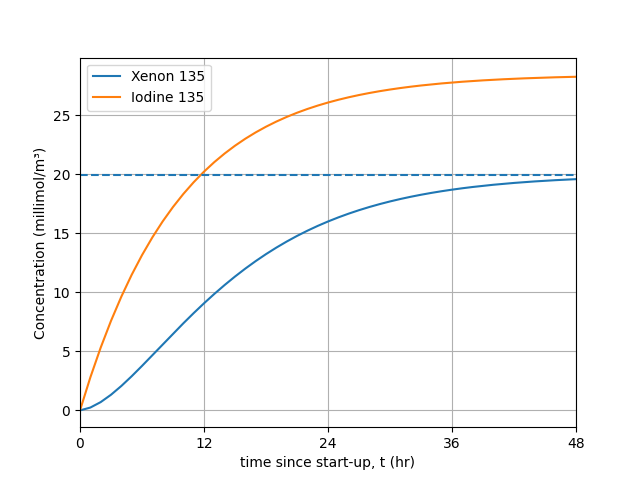
\includegraphics[width=0.75\textwidth]{Xenon/start-up}
    \caption[Concentration of \I and \Xe vs. time following start-up]{Concentration of \I and \Xe vs. time following cold/clean start-up. \I and \Xe are formed by fission as soon as the reactor starts. Soon after, \I decays to \Xe, and \Xe captures neutrons, being transmuted to \Xe[136]. These two species reach equilibrium values when generation and consumption are equal.}
    \label{fig:startup}
\end{figure}

\begin{figure}[ht!]
    \centering
    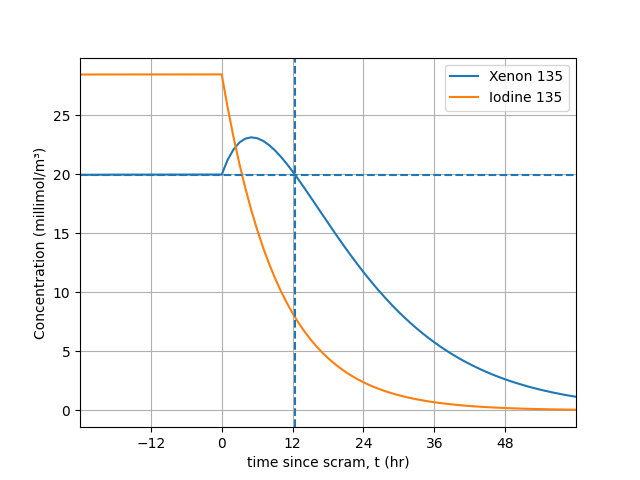
\includegraphics[width=0.75\textwidth]{Xenon/noHe}
    \caption[Concentration of \I and \Xe vs. time following reactor scram]{Concentration of \I and \Xe vs. time following reactor scram. When the reactor is scrammed, fission and transmutation cease. \I and \Xe each continue decaying. Initially, \I decays at a higher rate due to the shorter half-life and larger population. The \Xe concentration reaches its peak when the rate of \I decay drops below the rate of \Xe decay. After the equilibrium value is passed, the reactor may be restarted safely.}
    \label{fig:Control}
\end{figure}

The \Xe and \I concentration profiles during a clean start-up are depicted by \cref{fig:startup}. The \I level rises to an equilibrium concentration of 28.4 $\nicefrac{mmol}{m^3}$ as a first order response over the course of two days. The \Xe level follows an over-damped second order response to the its equilibrium level (denoted by the horizontal dashed line) of 20.0 $\nicefrac{mmol}{m^3}$. Using \ref{eq:Xe_poison}, equilibrium xenon accounts for -1.38\% of poison reactivity. The `shoulder' during the first few hours is formed because its primary source, precursor decay, is initially null. Similarly, the elongation of the curve is caused by the changing formation rate as the \I concentration rises. 

After \I and \Xe equilibrate, the reactor is scrammed by setting the prompt neutron flux to zero, subsequently producing the behavior shown in  \cref{fig:Control}. The \I concentration falls by simple exponential decay, while the \Xe concentration undergoes a second order response with numerator dynamics, peaking at 23.11 $\nicefrac{mmol}{m^3}$ 7 hours after the scram. The -1.60\% xenon reactivity at the peak represents a 16\% super-equilibrium. The \Xe concentration crosses its full power equilibrium 12.4 hours after the scram, which is denoted by a vertical dashed line. Delayed neutrons make a relatively small contribution over the hours following shutdown, decaying from 0.67\% to 1 ppm of the full power flux in under 8 minutes. Minimal impact to the \Xe concentration profile was estimated to be at the part-per-billion order by inspection of results with and without the delayed neutron subroutine.

\subsubsection{Verification of the Numerical Solver} 
For the given inputs, \ref{eq:I_eq} and \ref{eq:Xe_eq} predict an equilibrium \I concentration of 28.4 $\nicefrac{mmol}{m^3}$, and an equilibrium \Xe concentration of 19.96 $\nicefrac{mmol}{m^3}$. \ref{eq:Xe_peak} predicts that the peak of the inverse response occurs 5.1 hours and 3 minutes after the reactor is scrammed, with a magnitude of 23.1 $\nicefrac{mmol}{m^3}$ obtained by inserting the peak time into \ref{eq:Xe_bateman}. The analytic solutions of characteristic stationary points of the system of \acsp{ode} give identical results with respect to the numerical solver, verifying the results of the model for the benchmark study.

To further verify the numerical solver, the path by which nuclide concentration approaches equilibrium can be compared to analytical solutions. By making the simplification of constant (time-independent) neutron flux, an analytical solution can be obtained for the \I concentration:
\begin{equation}\label{eq:I_analytical}
\left.I(t)\right\rvert_\phi = (I_o-I_\infty)e^{-\lambda_I t}+I_\infty
\end{equation}

The accuracy of the numerical solver was quantified by comparing the \I concentration array to \ref{eq:I_analytical}. An $1-r^2$ score of $1.46\times10^{-8}$ was obtained over the first 48 hours of start-up. This value is not sensitive to the initial condition, with approximately the same $r^2$ value being observed regardless of the \I level at start-up. This was tested over a range from 10\% to 5 times the equilibrium value.

The \Xe rise to equilibrium is more difficult to analytically solve, owing to the variable generation rate caused by the changing decay rate of \I. Because $I_\infty$ is already known, we can choose this as $I_o$, which makes the \I concentration and \Xe generation rate constant at $\gamma_{Xe}\Sigma_{f}^{F}{\phi}$ and the ODE separable. This is not a physically meaningful calculation, but it does hold mathematical meaning, and the solver is capable of computing it. The solution to this simplified ODE has the same form as \ref{eq:I_analytical}, with the effective decay constant, $\lambda_{Xe}+\sigma_a^{Xe}\phi$, in the exponent. By replicating the assumptions of the simplified ODE, the numerical solver was found to have an $r^2$ value of essentially 1. During normal operation of the solver, some error propagation is expected which would cause the numerical \Xe solution to be slightly less precise. However the low error calculated in the \I verification limits the effect of error propagation.

The \I verification gives assurance that the fission yield and beta decay methods work as intended, while the \Xe scenario verifies the radiative capture method. To verify the precursor decay method, \ref{eq:I_bateman} and \ref{eq:Xe_bateman} are compared to the numerical solutions, obtaining $1-r^2$ scores of $1.05\times10^{-9}$ and $4.59\times10^{-10}$. The level of precision achieved by the numerical solver in the verification studies gives confidence that it will accurately predict the behavior in more complicated studies, for which analytical solutions are difficult to obtain.

\subsubsection{Super-Equilibrium Restart}
The first experiment was repeated, but this time the reactor was restarted at the xenon peak, producing the behavior shown in \cref{fig:PeakRestart}. 96 pcm of \Xe burned out in the first hour, and the \Xe reactivity dipped to 120 pcm below its equilibrium level 10.4 hours after the reactor was restarted. 

\begin{figure}[ht!]
    \centering
    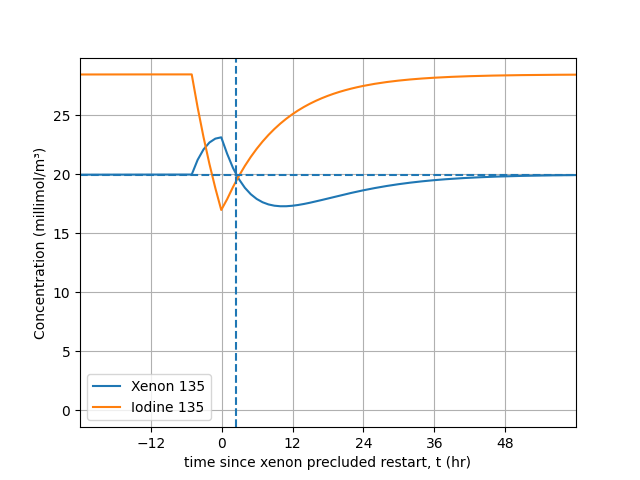
\includegraphics[width=0.75\textwidth]{Xenon/peakrestart}
    \caption[Concentration of \I and \Xe vs. time following restart at xenon peak]{Concentration of \I and \Xe vs. time following restart at xenon peak. When the reactor is restarted, fission and transmutation resume. \I immediately builds back up, while \Xe burns out, returning to equilibrium after a substantial overshoot.}
    \label{fig:PeakRestart}
\end{figure}

This is a significant disturbance to the poison reactivity of the reactor during operation. The magnitude of the reactivity swing during the restart is equivalent to 25\% of the difference between clean start-up and equilibrium xenon poisoning, and the maximum burnout rate is more than 1.5 times the maximum \Xe build-up rate during initial start-up (63 pcm/hr). The most significant issue is that the burn-out of super-equilibrium \Xe during operation causes a positive feedback loop that the reactivity controller has to reject; if the drop in poison reactivity is not counteracted by control rod insertion, the neutron population grows, which increases the xenon burn-out rate.

With proper reactor and controller design, this disturbance can be managed. With a temperature coefficient of 3.5 pcm/K, the core temperature could swing by up to 27 degrees Celcius in the first hour, and 97 degrees overall \cite{CarterMCNP}. Depending on the hot standby temperature, coolant salt volatility limits could be approached. More likely, downstream systems such as power cycles and process heat applications may be disturbed, putting stress on the plant-wide distributed control system. While this may be manageable, it would be preferable, and potentially required, to avoid this type of re-start.

\subsubsection{Scheduled Restart}
An \acs{msr} deployed in a load-following capacity on an isolated grid may at times need to be shut down (or ramped down) overnight, then be powered up in the morning. The numerical solver was used to study such a scenario plotted in \cref{fig:Restart}. The \I concentration decays as in \cref{fig:Control}, and the \Xe concentration rises initially. Due to the stripping term in \ref{eq:diffXe_strip}, the peak is lower and occurs sooner, and the poison level crosses the equilibrium value sooner. The flow rate ratio ($\frac{\dot{V}_{He}}{\dot{V}_{salt}}$) required to return the \Xe concentration to its equilibrium value after 8 hours of dead-time is $2.15 \times 10^{-7}$. This corresponds to just 2.1 $\nicefrac{mL}{hr}$ of helium, or 16.8 mL over the entire dead-time. At approximately atmospheric pressure and 1000 K, this is such a small amount of helium that, if single-stage equilibrium is practically achievable, it may make more sense to release all of the necessary helium in a single pulse or series of pulses over the dead-time rather than continuously.

\begin{figure}[b!]
    \centering
    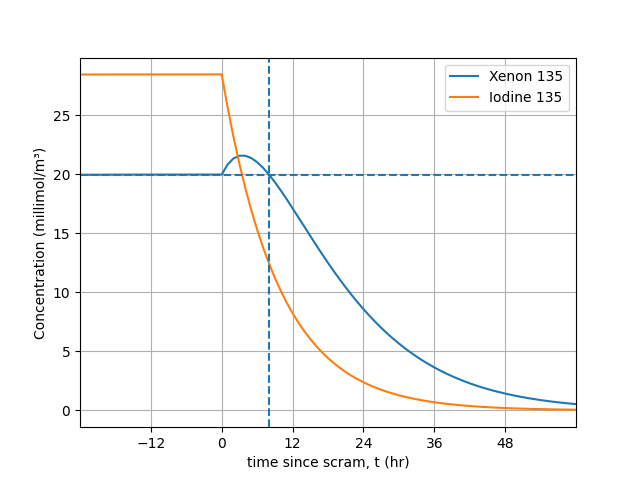
\includegraphics[width=0.75\textwidth]{Xenon/8hr_restart}
    \caption[Concentration of \I and \Xe vs. time following reactor scram - Restart Mode]{Concentration of \I and \Xe vs. time following reactor scram with Xenon Stripping Module. The same dynamics take place as in \cref{fig:Control}, except in this case the \Xe is also being removed from the molten salt fuel in the Xenon Stripping Module, so the reactor may be restarted in 8 hours.}
    \label{fig:Restart}
\end{figure}

Such a pattern may fit into the energy demands of a modest island population, for example Guam, where much less power is required overnight. Conventionally this would not be feasible as it would require powering up from hot-standby or low-power mode during the xenon peak. A xenon stripping module could be coupled to the reactor to shorten the super-equilibrium time period, and make it possible to produce electricity on schedule.

A more traditional method for accelerating the effective half-life below what is achieved by beta decay alone, is low power burn-out. Maintaining the shut-down reactor at 1\% power, which is on the order of the thermal power from decay heat, can reduce the effective half-life to 9.11 hours (compared to the half-life of 9.21 for pure beta decay). In comparison, the usage of the xenon stripper outlined in this experiment yields an effective half-life of 7.29 hours. This represents a 25 fold increase in the effectiveness of \Xe removal.

\subsubsection{Demand Response}
Power-peaking is another dynamic energy sector that must be decarbonized. An \acs{msnb} acting in this capacity will need to be able to black-start within minutes of a call for power. To return the \Xe concentration from its peak at 7.0 hours after shut-down to its equilibrium level in 390 seconds (3 hot-standby flow periods) requires a helium flow rate of 2.9 $\nicefrac{mL}{min}$, totalling 19 mL over the entire start-up procedure. \cref{fig:Standby} displays the \I and \Xe as calculated by the numerical solver with these settings. It is identical to \cref{fig:Control} until the peak poison level, when the xenon stripping module is activated and the \Xe level drops rapidly. 

If this standby restart was conducted every day for 10 years, it would require only 1 mole of helium gas. This is a conservative estimate due to the short duration that the xenon-stripping module is active. The solver instantly distributes the effect of the stripped xenon across the entire reactor. This prematurely depresses the mass transport driving force and therefore predicts a lower separation efficacy than would be observed in practice. Expansion of the solver to a 1D+time or multi-region lumped parameter model could improve the accuracy for this case study, at the expense of significanty more computational expense.

\begin{figure}[ht!]
    \centering
    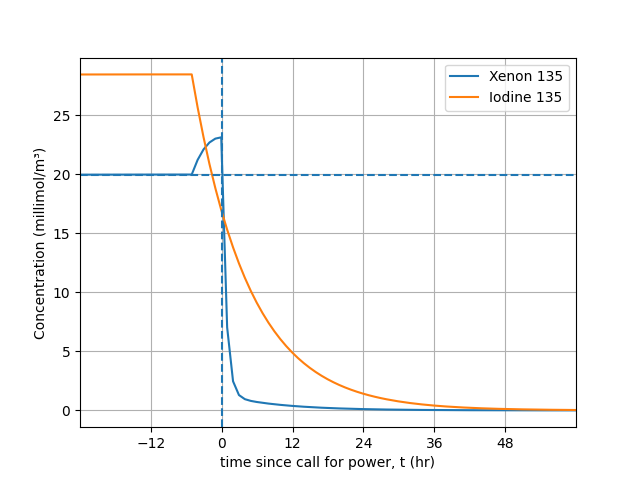
\includegraphics[width=0.75\textwidth]{Xenon/standby_restart}
    \caption[Concentration of \I and \Xe vs. time following reactor scram - Standby Mode]{Concentration of \I and \Xe vs. time following reactor scram with Xenon Stripping Module operating only immediately after the \Xe concentration reaches its peak. The same dynamics take place as in \cref{fig:Control}, except in this case \Xe is rapidly stripped from the molten salt fuel immediately after the \Xe concentration reaches its peak.}
    \label{fig:Standby}
\end{figure}

\newpage
Operators of an \acs{msr} that is implemented in a power-peaking application will not know exactly when it needs to be restarted, but will need to have the reactor on standby. If this is the case, the xenon stripping module could remain off until the start-up signal comes. The module could then operate at a much higher helium flow rate than seen in the previous experiment for a short period of time similar to the start up time of our current natural gas peaking generators \cite{GE} before the \acs{msnb} is black-started. 

\subsubsection{End of Life Fuel}\label{sec-EOL}
 Molten salt microreactors such as the \acs{msnb} could extend their lifetime with xenon stripping. At the end of the fuel lifetime, excess reactivity could be reclaimed by constantly removing \Xe from the fuel, driving down the equilibrium concentration. A helium flow rate of 146 mL/hr reduces the equilibrium poison reactivity from 1.38\% to 0.15\%, a reduction of 1227 pcm. \cref{fig:EOLstartup} displays that the \I concentration is unchanged with respect to \cref{fig:startup}, while the \Xe concentration is greatly depressed. 
 
 Equilibrium xenon accounts for a significant amount of poison reactivity at high power density. Because microreactors are small, they are often limited in excess reactivity. They are also often designed to last upwards of a decade without refueling. For an \acs{msnb} with approximately 5\% excess reactivity at initial start-up, \Xe poisoning greatly reduces the fuel lifetime. A reduction in the equilibrium poison level such as the one described in this experiment requires 1270 L of helium per year, but could conceivably extend the overall reactor lifetime by up to 30\%.
This result alone, without considering the effect of shortening restart time, makes the xenon stripper an important design feature to small \acsp{msr}, which are competing for a market share in a class of reactors that are aiming for decade scale operation \cite{PetersonMS}.

\begin{figure}[ht!]
    \centering
    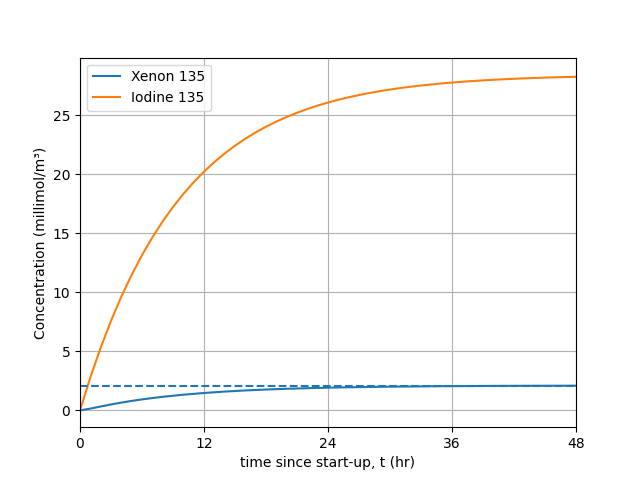
\includegraphics[width=0.75\textwidth]{Xenon/EOL-startup}
    \caption[Concentration of \I and \Xe vs. time during start-up - End of Life Fuel Mode]{Concentration of \I and \Xe vs. time during reactor start-up with Xenon Stripping Module operating to lower the equilibrium \Xe concentration.}
    \label{fig:EOLstartup}
\end{figure}


\section{Future work} \label{sec-fwk}
This work is a computational screening of xenon stripping for neutron poison management on a generic \acs{msr}, both during operation and during brief shut-down periods. Furthermore, it contains the development of a preliminary design tool that can be used to advise decisions in the specific design of \acsp{msr}. Many assumptions were made, notably a constant Henry's Law coefficient, which is subject to change during operation due to changing composition, and a constant natural circulation flow rate. These assumptions were made because of the lack of experimental data and the effect of design specifications on these parameters. By making the solver open source, we encourage other researchers to refine these assumptions as progress in experimental work supports.

\subsection{Xenon Stripping Module}
This paper works on the simplifying assumption that the xenon stripping module is an equilibrium mass transport unit operation. It has been demonstrated that the thermodynamics of \Xe stripping from molten salt fuel are highly favorable due to xenon's noble gas nature. This warrants a more detailed investigation into the kinetics of the unit operation. Literature must be consulted to design such a module \cite[Ch. 10]{Geankoplis}. It is highly likely that a higher helium flow rate will be required to prevent flooding and result in a sufficient interfacial area to volume ratio for mass transport to occur at any meaningful macroscopic rate. 

This paper also neglects the effect of other fission gasses that will be produced in the core, namely tritium. Core burn-up modeling will need to be conducted, and literature reviewed to see what other gasses may be stripped \cite{Offgas}. These additional gasses may inhibit xenon stripping by effecting the mass transfer coefficient, but will more likely facilitate improved stripping by contributing to the formation of circulating voids which may be removed from the salt more readily \cite{XeMSR}. 

\subsection{Numerical Solver}
The numerical solver is an object oriented program, making it modular. The architecture supports the instantiation of additional nuclides with a minimal amount of extra code. It could be used to study other equilibrium poison systems such as the \Sm decay chain, burnable poisons like gadolinium isotopes, and non-burnable poisons like hafnium isotopes. Outside of neutron poisoning, the solver could be modified to optimize isotope production schemes, track the gamma-ray source strength or decay heat potential of irradiated materials, or even estimate radiation damage and fission product interaction.

The solver is faster than real-time. A potential application beyond preliminary design is in control systems. A similar architecture could be employed to develop reduced-order just-in-time digital twins which would advise supervisory controllers during transient operations. This would allow, for example, the control system of a nuclear reactor to account for poison reactivity changes without having to wait for the disturbance to cause a set-point error, as would be required in a pure feedback controller.



\section{Conclusions} \label{sec-sum}
A new model was derived that quantifies the advective removal rate of \Xe from a molten salt fuel in an equilibrium stripper using Henry's law constants obtained from literature. It was used to demonstrate that, given appropriate conditions, mass transport can strongly outweigh beta decay in the post shutdown \Xe decay chain dynamics. Results show that a bulk gas stream on the order of milliliters provides enough volume for nearly all of the \Xe in a liter of molten salt fuel to transport into the gas phase. The challenge now shifts from providing sufficient volume to do this, to providing sufficient interfacial area; this paper shows that this problem is worth solving. If solved, this technology opens the door to \acsp{msr} breaking into remote grids and power peaking.




% -- Reactor Characterization --
\chapter{Reactor Characterization}
\label{Chapter:Modeling}
To design a reactivity controller for the \acl{msnb}, many components of the reactor needed to be characterized. The reactor was modeled in Serpent 2 to characterize the control drums using a series of criticality models. Depletion models were also used observe how the control drum characterization changes as the fuel is burned. Finally, a 1-dimension (spatial) uniform-state uniform-flow finite element model was developed in Python. This serves as the thermohydraulic process simulation needed to approximate the autonomous dynamic operation of the reactor during transients as well as study the performance improvement gained by application of the controller. 

\begin{figure}[!ht]
    \centering
    \resizebox{\textwidth}{!}{
\begin{tikzpicture}
    %Pre-filter
    \draw[->] (-6,0)node[anchor=east]{$\dot{Q}_{HEX}$} -- (-4.5,0);
    \draw (-4.5,-0.5) rectangle (-3.5,0.5) node[pos=0.5]{$F(s)$};
    %Sum
    \draw[->] (-3.5,0) -- (-2,0) node[pos=0.5,anchor=south]{$\dot{Q}_{Core}^{SP}$};
    \draw (-1.75,0) circle (0.25) node{\scriptsize$\textbf{-}$};
    %Controller
    \draw[->] (-1.5,0) -- (-0.5,0)node[pos=0.5,anchor=south]{$e$};
    \draw (-0.5,-0.5) rectangle (0.5,0.5) node[pos=0.5]{$C(s)$};
    \draw[->] (0.5,0) -- (1.5,0) node[pos=0.5,anchor=south]{$u_{CD}$};
    %Actuator
    \draw (1.5,-0.5) rectangle (2.5,0.5) node[pos=0.5]{$A(s)$};
    \draw[->] (2.5,0) -- (3.5,0) node[pos=0.5,anchor=south]{$\rho_{CD}$};
    %Sum
    \draw (3.75,0) circle (0.25) node{\scriptsize$\textbf{+}$};
    %Process
    \draw[->] (4,0) -- (5,0) node[pos=0.5,anchor=south]{$\rho$};
    \draw (5,-0.5) rectangle (6,0.5) node[pos=0.5]{$P(s)$};
    \draw[->] (6,0) -- (8,0) node[anchor=west]{$\dot{Q}_{Core}$};
    %Transducer
    \draw[->] (7,0) -- (7,-1.5) -- (2.5,-1.5);
    \draw (1.5,-2) rectangle (2.5,-1) node[pos=0.5]{$H(s)$} ;
    \draw[->] (1.5,-1.5) -- (-1.75,-1.5) -- (-1.75,-0.25);
    %Passive Feedback
    %Core Feedback
    \draw[->] (7,0) -- (7,2.5);
    \draw (6.5,2.5) rectangle (7.5,3.5) node[pos=0.5]{$G_{C}(s)$};
    \draw[->] (6.5,3) -- (4.25,3);
    %HEX Feedback
    \draw[->] (-5,0) -- (-5,2.5);
    \draw (-4.5,2.5) rectangle (-5.5,3.5) node[pos=0.5]{$G_{H}(s)$};
    \draw[->] (-4.5,3) -- (3.25,3)node[pos=0.5,anchor=south]{$T_{cold}$};
    %Sum
    \draw (3.75,1.5) circle (0.25) node{\scriptsize$\textbf{+}$};
    \draw[->](3.75,1.25) -- (3.75,0.25);
    %TemperatureFeedback
    \draw (1.5,1) rectangle (2.5,2) node[pos=0.5]{$\alpha_T$};
    \draw[->] (2.5,1.5) -- (3.5,1.5) node[pos=0.5,anchor=south]{$\rho_{T}$};
    %FlowFeedback
    \draw (3.25,2.5) rectangle (4.25,3.5) node[pos=0.5]{$\alpha_F$};
    \draw[->] (3.75,2.5) -- (3.75,1.75) node[pos=0.5,anchor=west]{$\rho_{F}$};
    %Downcomer
    \draw[->] (0,3) -- (0,2);
    \draw (-0.5,1) rectangle (0.5,2) node[pos=0.5]{$\theta_{DC}$};
    \draw[->] (0.5,1.5) -- (1.5,1.5);
    %Riser
    \draw[->] (5.375,3) -- (5.375,4.5) -- (0.5,4.5) node[pos=0.5,anchor=south]{$T_{hot}$};
    \draw (-0.5,4) rectangle (0.5,5) node[pos=0.5]{$\theta_{R}$};
    \draw[->] (-0.5,4.5) -- (-5,4.5) -- (-5,3.5);


\end{tikzpicture}
}
    \caption[Control loop of a natural circulation \acs{msnb}]{Control loop of a natural circulation \acs{msnb}. It is a normal feedback loop with a pre-filter, with the addition of the passive feedback mechanisms. The core ($\dot{Q}_{Core}$) and heat exchanger ($\dot{Q}_{HEX}$) powers go through the respective temperature dynamics ($G_C$ and $G_H$) and time delays for the riser ($\theta_R$) and downcomer ($\theta_{DC}$) before being converted to reactivity by the temperature($\alpha_T$) and flow ($\alpha_F$) feedback mechanisms. The passive reactivity feedback is combined with the control drum reactivity ($\rho_{CD}$) and fed into the reactor dynamics ($P(s)$).  }
    \label{fig:ReactorControlLoop}
\end{figure}

\section{Reactor Design}\label{Section:Design}
The \acs{msnb} is self contained in a 145 cm diameter, 242 cm tall cylindrical rector vessel that is buried in the ground or concrete for shielding purposes. The core is a concentric 166 cm tall cylinder 50 cm in diameter surrounded by a large reflector into which 8 equally spaced control drums are embedded. A neutron trap sits above the reflector to separate the riser, where fission caused by delayed neutrons occurs at a significant rate, from the heat exchanger. The downcomer is an annular gap between the outer part of the reflector and the outer reactor vessel. It has flow area identical to the core, and returns cold salt from the outlet of the heat exchanger to the inlet plenum.

Figure \ref{fig:Plotter-YZ} is an axial cross-section of the \acs{msnb}. Figure \ref{fig:Plotter-XY} contains four radial cross-sections of the \acs{msnb}. These two figures were generated by the Serpent model described in Section \ref{Section:Serpent}. In these models, \UF dissolved in \flinak is depicted as varying shades of red depending on temperature, beryllium-oxide is light-blue, boron-carbide is green, graphite is yellow, stainless steel is light-gray, Hastelloy-N is medium-gray, barite concrete is dark-gray, and air is pink. The reactor is buried in barite concrete for radiation shielding purposes, and the top is at the surface so secondary coolant systems can readily be connected.

\begin{figure}[ht!]
    \centering
    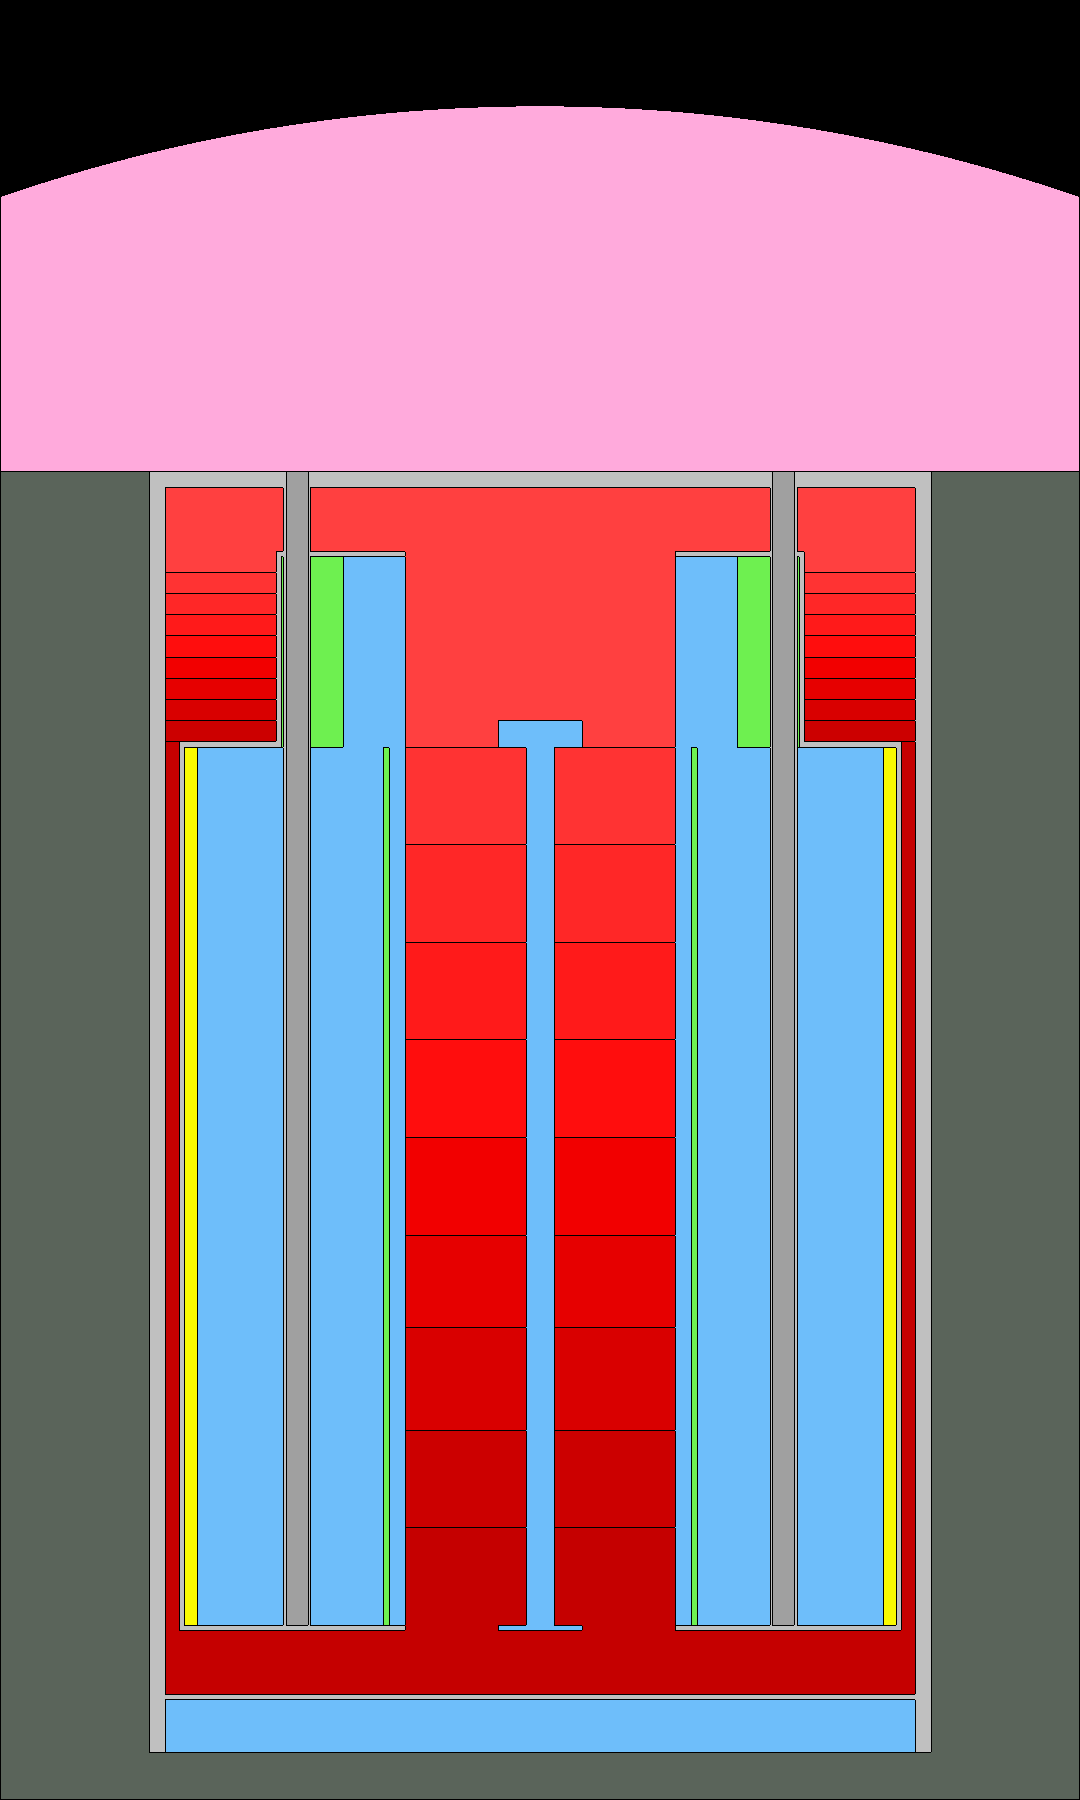
\includegraphics[width=0.75\textwidth]{Plotter/0.0/MSNB_geom1.png}
    \caption[Y-Z view of \acs{msnb}]{Y-Z view of \acs{msnb}. Molten salt is shown in red, with darker shades corresponding to a lower temperature and higher density. The core is surrounded by the beryllium-oxide reflector (blue) and the boron-carbide absorber plate (green). The core is separated from the riser by a a perforated reflector plate and the riser is separated from the heat exchanger by an absorbing ring. From this angle the internal moderating structure appears as only the center rod, as the fins exist in other planes.}
    \label{fig:Plotter-YZ}
\end{figure}
\clearpage
\begin{figure}[!ht]
    \centering
    \subfloat[\centering Inlet Plenum]{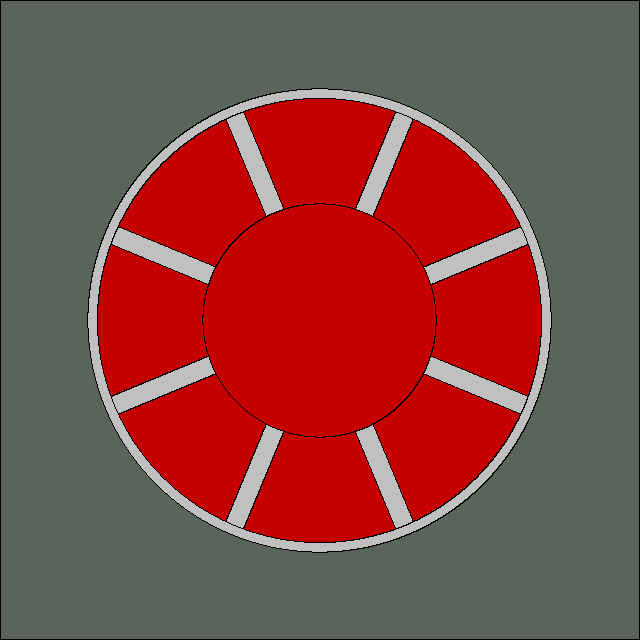
\includegraphics[width=0.49\textwidth]{Plotter/0.0/MSNB_geom2}}
    \subfloat[\centering Core]{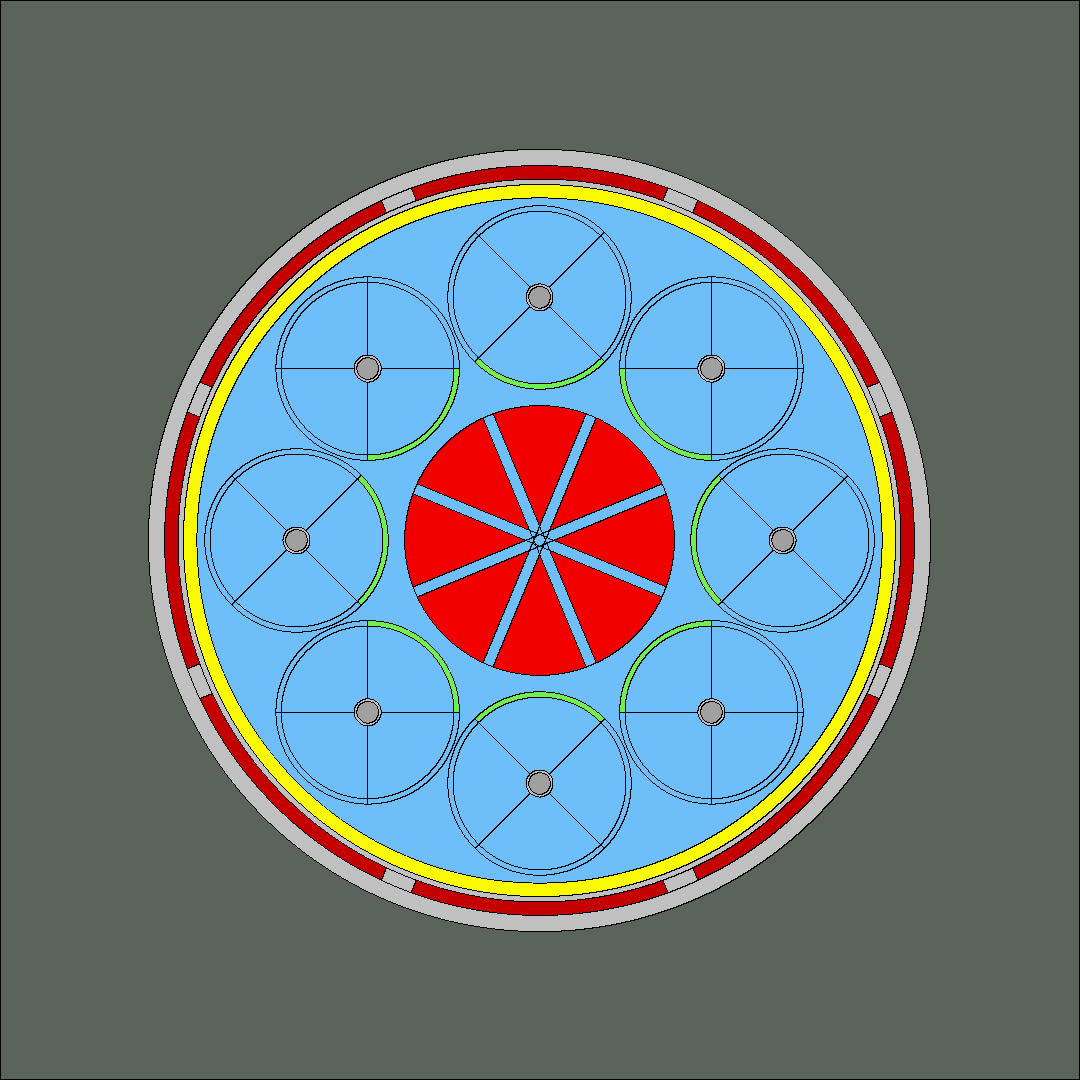
\includegraphics[width=0.49\textwidth]{Plotter/0.0/MSNB_geom4}}
    \quad
    \subfloat[\centering Heat Exchanger]{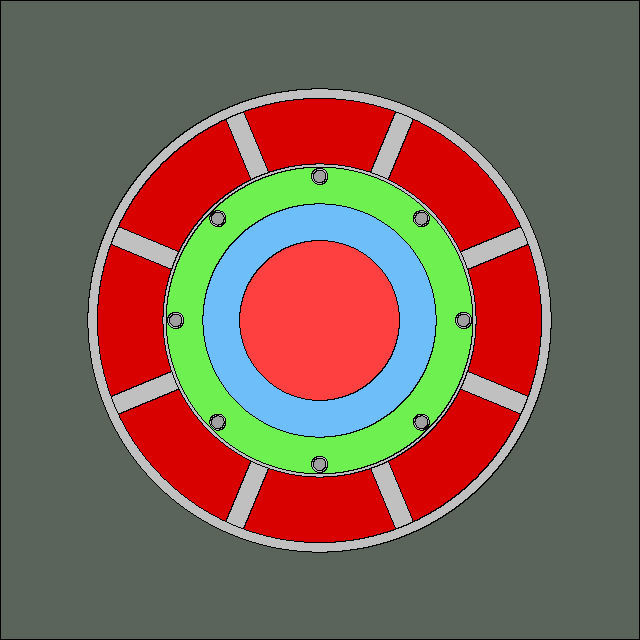
\includegraphics[width=0.49\textwidth]{Plotter/0.0/MSNB_geom6}}
    \subfloat[\centering Spoke]{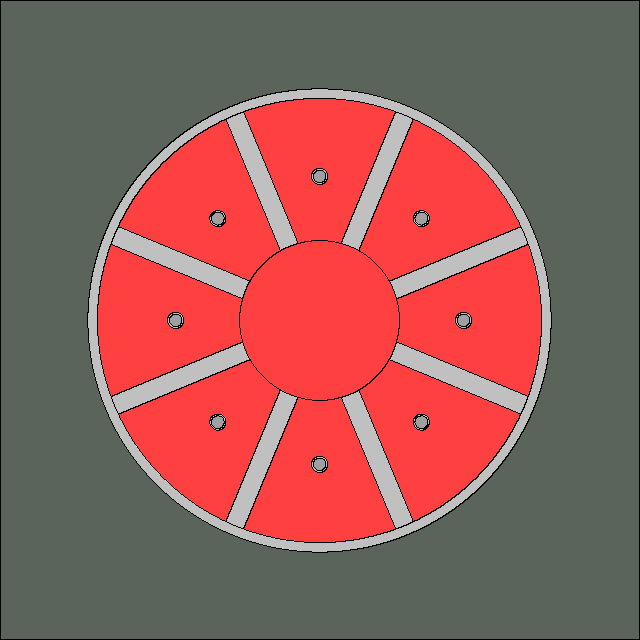
\includegraphics[width=0.49\textwidth]{Plotter/0.0/MSNB_geom8}}
    \caption[X-Y Views of \acs{msnb}]{X-Y Views of \acs{msnb}
    \begin{enumerate*}[label=\alph*)]
        \item Molten salt from the downcomer travels inward below the reflector the center, where it rises to enter the core;
        \item The core is surrounded by the reflector and control drums, which may be adjusted to manipulate criticality. The reflector and downcomer are separated by a graphite shield;
        \item The molten salt in the outer ring is in the heat exchanger. As it sinks, heat is being rejected to the secondary coolant (not modeled). A ring of boron-carbide ensures that delayed neutrons emitted in the riser do not transport to the heat exchanger; 
        \item Molten salt exiting the riser travels radially outward to the top of the heat exchanger;
    \end{enumerate*}}
    \label{fig:Plotter-XY}
\end{figure}

\subsection{Molten Salt}
The molten salt in the \acs{msnb} serves as both the primary coolant and the fuel. It is composed of 18 mol\% \acs{haleu} \UF \; (enriched to 19.75\%) dissolved in eutectic \flinak (enriched to 99.99\% \Li[7]). It is composed of about 1.4 atom\% \U[235]. The remaining composition is listed in Table \ref{tab:saltcomp}. This molten salt fuel system has been studied in previous work \cite{CarterPHD}. The present work leverages intermediate calculations, such as the thermophysical property temperature functions - density\footnote{note the use of $\varrho$ to distinguish density from reactivity ($\rho$)} ($\varrho$) and heat capacity ($c_p$) - of the salt:

\begin{equation}\label{eq:saltdens}
    \varrho[kg/m^3] = 4682.0365 - 0.94301046\cdot T[K] 
\end{equation}
\begin{equation}\label{eq:saltcp}
    c_p[kJ/kg-K] = 0.97678 + 0.0010634\cdot T[K]
\end{equation}

\flinak was selected for study due to its thermal properties and prevalence in \acs{msr} research, and \UF \; was selected as it is soluble in \flinak to a concentration that has a wide liquidus range, supports criticality in the reactor geometry necessary to fit into a shipping container, and provides adequate power density for thermal hydraulic design. 

\begin{table}[ht!]
    \caption[Molten salt composition]{\raggedright Composition of molten salt prior to burn-up}
    \centering
    \begin{tabular}{rl|cc}
     Element&Isotope&Atom Percent & Weight Percent \\ \hline
     Fluorine  & 19  & 60.63 \%  & 32.40 \% \\  \hline
     Lithium   & 6   & 15 ppm    & 2.5 ppm  \\
               & 7   & 15.01 \%  & 2.96 \%  \\ \hline
     Sodium    & 23  &  3.71 \%  & 2.40 \%  \\ \hline
     Potassium & 39  & 12.61 \%  & 13.82 \% \\
               & 41  & 0.95 \%  & 1.09 \%  \\ \hline
    Uranium    & 235 & 1.40 \%   & 9.25 \%  \\
               & 238 & 5.69 \%   & 38.08 \% \\
    \end{tabular}
    \label{tab:saltcomp}
\end{table}

\subsection{Control Drums}
Control drums are cylinders of neutron reflector with a portion of the circumference replaced with a neutron absorber. As is depicted by Figure \ref{fig:Plotter-CD}, rotating the control material inward inhibits the neutron chain reaction. This concept is used in the Advanced Test Reactor at \acs{inl}, using a beryllium/hafnium design \cite{atr}. It is also a popular concept for accident tolerance in space reactors, which have the potential to crash during launch \cite{AT-CD}. 

\begin{figure}[!ht]
    \centering
    \subfloat[\centering Least Reactive]{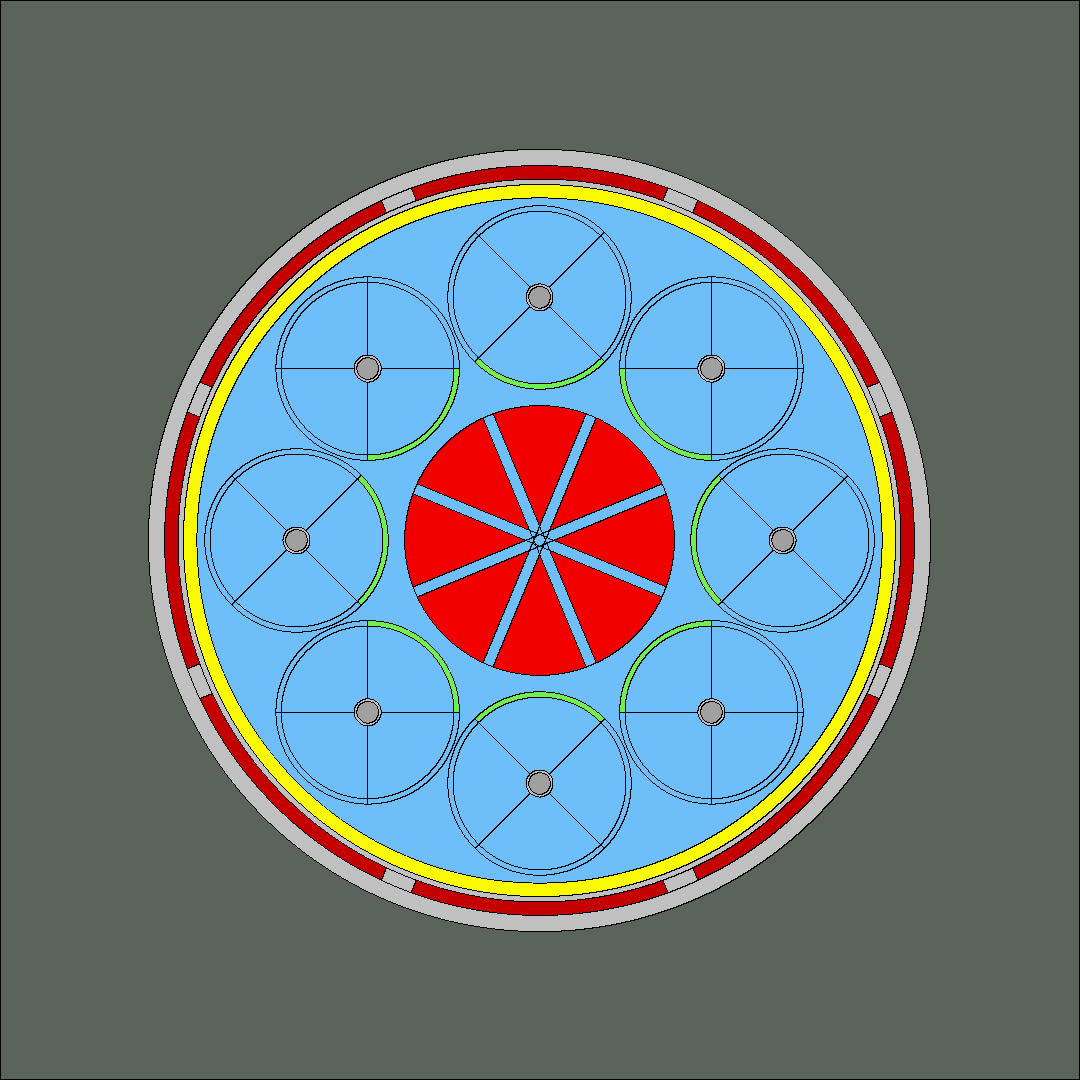
\includegraphics[width=0.33\textwidth]{Plotter/0.0/MSNB_geom4}}
    \subfloat[\centering Initial Criticality]{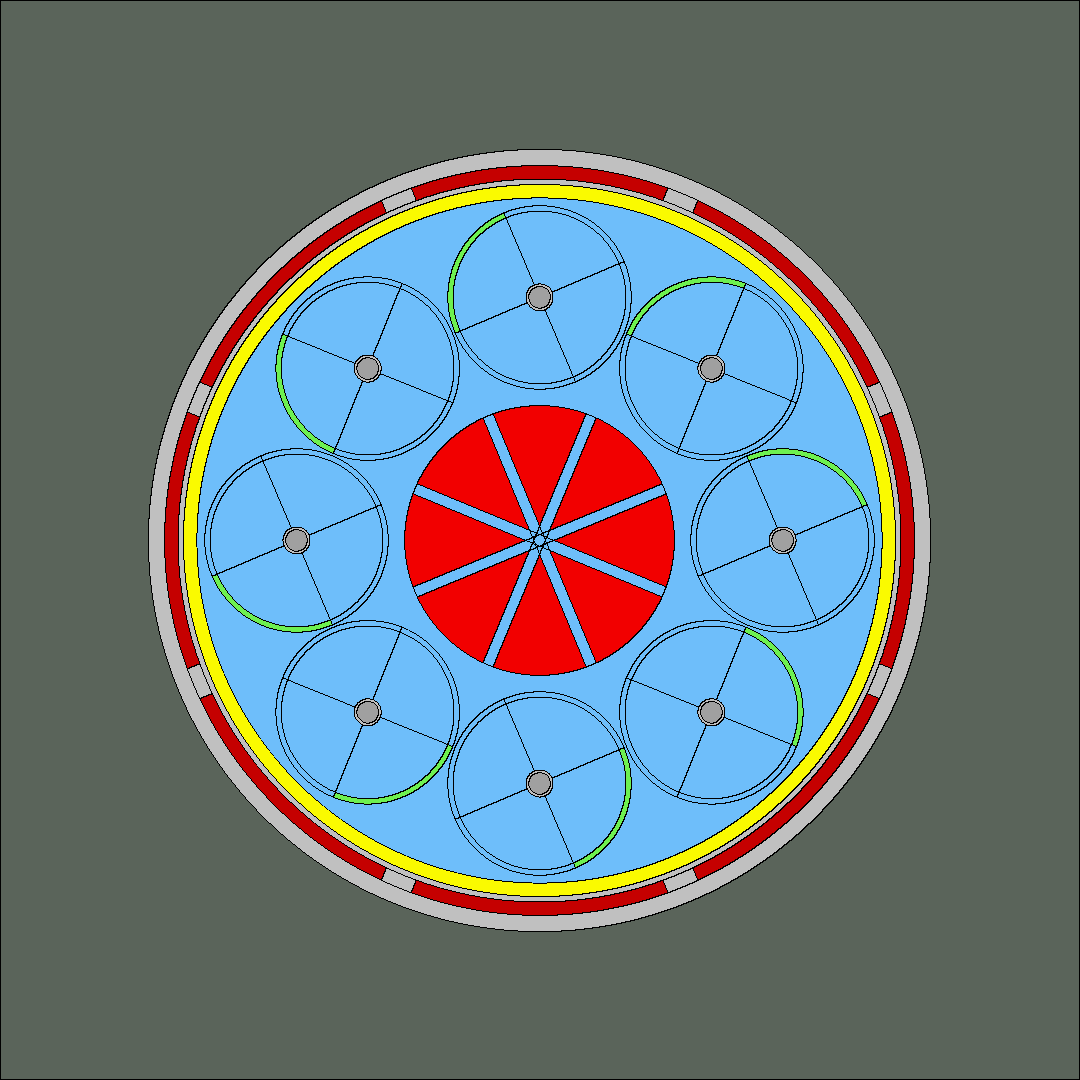
\includegraphics[width=0.33\textwidth]{Plotter/112.0/MSNB_geom4}}
    \subfloat[\centering Most Reactive]{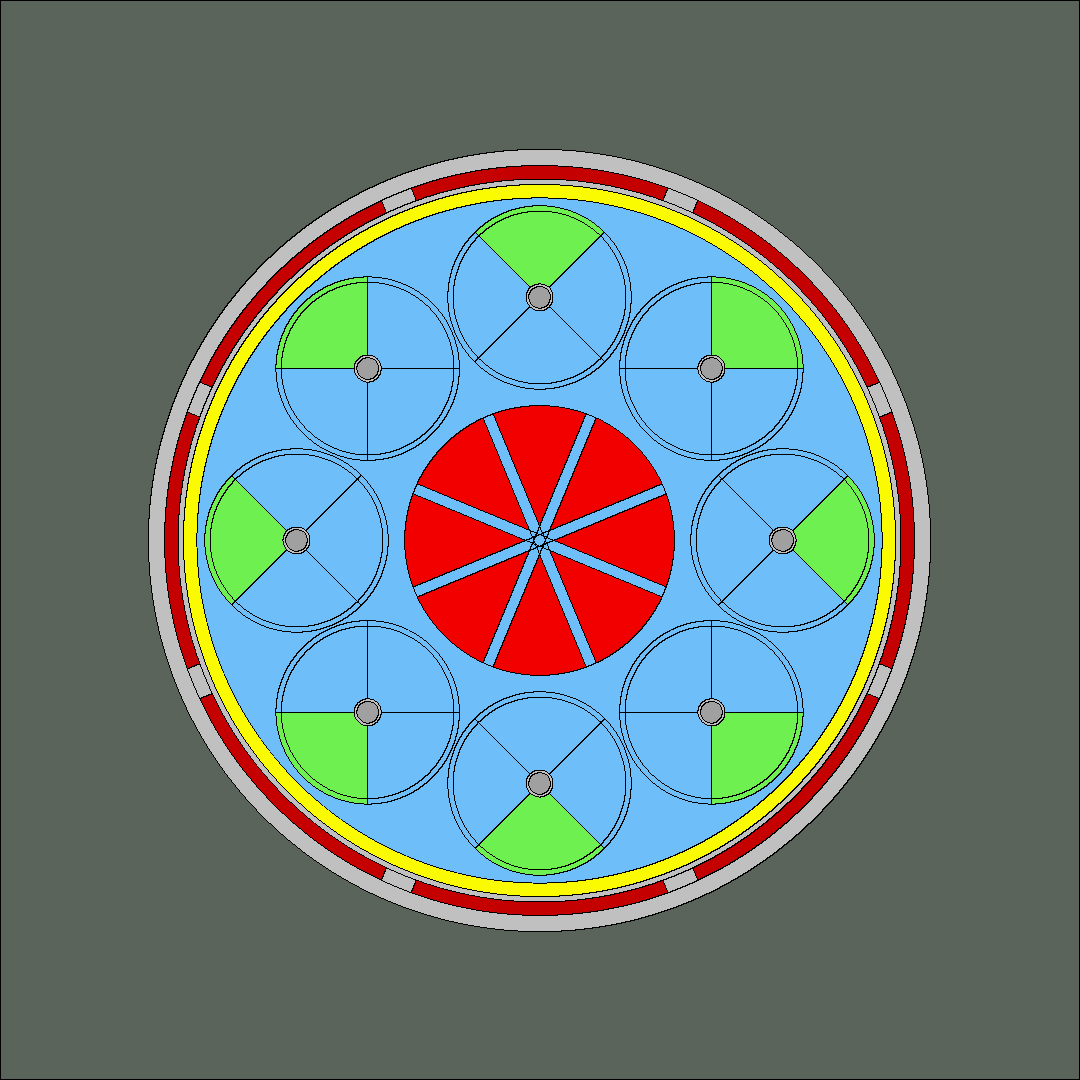
\includegraphics[width=0.33\textwidth]{Plotter/180.0/MSNB_geom4}}
    \caption[X-Y View of \acs{msnb} - Control Drums]{X-Y Views of \acs{msnb} with control drums in three orientations:
    \begin{enumerate*}[label=\alph*)]
        \item 0 degrees, which is used to test the reactor's shutdown margin;
        \item 112 degrees, which is the initial critical orientation; and 
        \item 180 degrees, which is used to test the reactor's excess reactivity; 
    \end{enumerate*}
    Beryllium oxide is depicted in blue while boron carbide is green. The entire wedge of each control drum is colored for clarity. Only the outer rim is actually made from boron carbide.}
    \label{fig:Plotter-CD}
\end{figure}

Each of the eight drums in the \acs{msnb} is the same height as the core, 17 cm in radius, and has a 1 cm thick absorber pad covering 25\% of the circumference. This study uses beryllium oxide as the reflector material for cost, machinability, and radiation damage considerations, and boron carbide for the absorber, as it provides adequate shutdown margin while preserving more excess reactivity than hafnium. 

In addition to the higher absorption cross-section, hafnium also is considered a non-burnable poison, as the transmutation products also have a high cross-section. In contrast, the products of \B[10] capture are essentially transparent to neutrons. It was confirmed using a burn-up study that the boron carbide would not be significantly depleted during the life of the \acs{msnb}.

\subsection{In-Pile Moderator}
Previous work has suggested an in-pile helix made of a neutron scattering material to extend the in core flow path and simultaneously soften the neutron energy spectrum to provide more excess reactivity \cite{CarterPHD}. This work investigates a simpler version of this concept focused only on providing excess reactivity. It is composed of 8 radial fins spaced 45 degrees apart, and is made from beryllium oxide.

\subsection{Structural Materials}
The reactor vessel, along with supplementary structural materials such as reflector and moderator supports, heat exchangers, and control drum driveshaft sheaths are made from 316 stainless steel. Control drum driveshafts are made from Hastelloy-N, a nickel-chromium-molybdenum alloy that is resistant to corrosion from high temperature fluoride salts. The reactor vessel is encased in barite concrete for added radiation shielding.

\section{Neutronics Modeling}\label{Section:Serpent}
The reactor described in Section \ref{Section:Design} was modeled in Serpent 2, making use of the Sawtooth supercomputer at \acs{inl}'s \acs{hpc} center. The fuel was stratified for an expected temperature rise using \ref{eq:saltdens} and redundant material cards. A python script was written to automatically generate the input cards that reflect a specific molten salt composition and control drum angle\footnote{The input file writing script is available at \href{https://github.com/sjroot97/MSNB-Serpent2-Autodeck}{https://github.com/sjroot97/MSNB-Serpent2-Autodeck} and is also included in Appendix \ref{app:Serpent}.} This made it easy to submit batches of several criticality models sequentially to Sawtooth using a Bash submission script.

 An alternating methodology of criticality and burn-up models was employed to characterize the control drums. First, the $k_{eff}$ for the entire range of control drum angles (from 0 to 180 degrees) was obtained using a criticality model that used 1,000,000 source particles per cycle, 500 active cycles, and 100 inactive cycles. With 32 nodes parallelizing 4 threads, each control drum angle took between 2 and 5 minutes to complete. This allowed the entire range of control drum angles to be simulated with a wall-time of 2 hours.  

 With the entire control drum angle vs. reactivity curve defined, the unity point was calculated and a burn-up model was conducted at that angle. A stochastic volume calculation was obtained using the `mcvol' subroutine, and the depletion module was loaded at 10 MW with a time-step of 6 hours until \Xe reached equilibrium, and 6 months following. Originally, smaller time-steps of 1-5 days were used to study the change to the control drum-reactivity curve as \Sm built up. This was forgone after finding that \Sm acts as a non-equilibrium fission product neutron poison at the relatively low power density studied. 
 
 To approximate the flowing and electrolytic nature of the \acs{msnb} that disperses fission products over time, the burn-up studies were completed without fuel stratification. This is in contrast to how solid fueled burn-up studies are often conducted, where depletion zones are employed to resolve the effects of the spatial neutron flux profile. This provided the new molten salt and boron carbide compositions for the next set of criticality models.

\section{Process Simulation}\label{Section:Python}
A multiphysics transient simulation was written in Python to study the \acs{msnb} in dynamic operations by the coupling of thermal hydraulics and neutronics. First principle physics were implemented to approximate the expected behavior of the reactor. It is not meant to be a digital twin, but rather a responsive tool for the design of the power controller\footnote{The input file writing script is available at \href{https://github.com/sjroot97/MsNB-Simulator/}{https://github.com/sjroot97/MsNB-Simulator/} and is also included in Appendix \ref{app:Simulator}.}.

The simulation is built on three physics principles: 
\begin{enumerate*}
    \item Thermally driven natural circulation flow mode, where the pressure differential driven by a difference in density between the hot and cold leg is equilibrated by frictional losses to calculate the flow rate;
    \item Reactor point kinetics, where the compound passive dynamics are used to time-advance the reactor power based; and
    \item Uniform-state uniform-flow time and spatial advancement of energy in the flow loop.;
\end{enumerate*}

\begin{figure}[ht!]
    \centering
    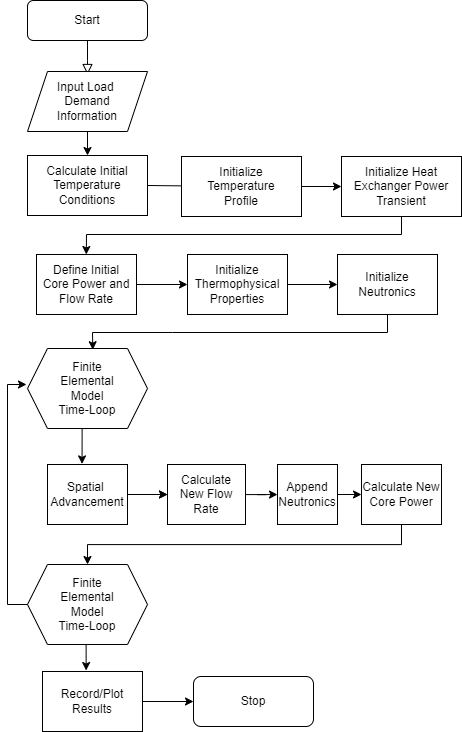
\includegraphics[width=0.5\textwidth]{FlowDiagram}
    \caption[Process simulator logic flow diagram]{\raggedright Logic flow diagram for the \acs{msnb} transient process simulator.}
    \label{fig:PythonFlowDiagram}
\end{figure}

Figure \ref{fig:PythonFlowDiagram} is a logic flow diagram that describes how the code simulates the dynamic operation of the \acs{msnb}. Similar to previous work, the flow loop of the reactor was simplified into a 1-dimensional flow loop with equal flow area throughout \cite{CarterNumerical,CarterPHD,Root}. The simulator is broken up into two different sections - first the problem is set-up, then the transient is simulated in a finite element time loop with time steps of 1 second. The model is described in Sections \ref{Section:initial} and \ref{Section:advance}, and rely on the parameters listed in Table \ref{tab:FEMparams}

\begin{table}[ht!]
    \caption[\acs{msnb} simulation parameters]{\raggedright System parameters used in the simulation of the \acs{msnb} \cite{CarterNumerical}. }
    \centering\begin{tabular}{r|ccl}
        &  Value &  Unit &  Description \\ \hline
    $\alpha_T$ & $-3.5$ & pcm/K & Temperature reactivity feedback coefficient \\
    $\ell^*$ & $1.63 \times 10^{-4}$  & sec & Mean neutron generation time \\
    $\beta_{eff}$ & $6.96 \times 10^{-3}$  & - & Effective delayed neutron fraction \\
    $\lambda$ & $0.1$  & sec$^{-1}$ & One-group delayed neutron precursor decay constant \\
    $\xi$ & $25$  & - & Pressure loss coefficient \\
    $h$ & $1.09$  & m & Height between thermal centers \\
    $\alpha_f$ & $-0.3398$ & s/cm & Flow reactivity feedback coefficient \\
    $A_x$ & $0.4$  & m$^{2}$ & Cross-sectional flow area \\
    $g$ & $9.81$  & m/s$^{2}$ & Acceleration due to gravity \\
    $\delta t$ & $1$  & sec & Time-step duration  \\
    $\delta x$ & $1$  & mm & Control volume length  \\
    \end{tabular}
    \label{tab:FEMparams}
\end{table}

\subsection{Model Initialization}\label{Section:initial}
The code first takes inputs to define the heat exchanger power transient that is to be studied. The reactor is initially assumed to be steady-state and critical, so the temperature is constant in the chimney and downcomer, and heating/cooling are uniform and equal in the core and heat exchanger. A binary search algorithm is used to iteratively find the cold leg ($T_{cold}$) temperature that corresponds to the initial power requirement with a hot leg temperature ($T_{hot}$) of 700 $^o$C. The heat exchanger power ($\dot{Q}_{HEX}$) is calculated by:

\begin{equation}
    \dot{Q}_{HEX} = \bar{\varrho}_{HEX} A_x v \bar{c_p}_{HEX} (T_{hot} - T_{cold})
\end{equation}

Where $\bar{\varrho}_{HEX}$ and $\bar{c_p}_{HEX}$ are the average density and heat capacity in the heat exchanger, $A_x$ is the cross-sectional flow area within the reactor, and $v$ is the velocity of the salt in the loop. The key assumption for this model is that the flow velocity during a given time-step is uniform throughout the flow loop, both during steady-state and unsteady-state time periods. This assumption allows for a simple spatial advancement, and an explicit total energy balance solution, which is described in detail in Section \ref{Section:advance}. The flow velocity is calculated based on the temperature profile, assuming a natural circulation flow mode:

\begin{equation}\label{eq:saltvelo}
    v = \sqrt{\nicefrac{2gh(\varrho_{cold}-\varrho_{hot})}{\xi\varrho}}
\end{equation}

where $g$ is the gravitational acceleration, $h$ is the height between thermal centers, $\xi$ is the pressure loss coefficient (estimated to be 25.0 by STAR-CCM+ \cite{CarterNumerical}), $\bar{\varrho}_{cold}$ and $\bar{\varrho}_{hot}$ are the average salt densities of the cold and hot leg, and $\bar{\varrho}$ is the average salt density of the entire reactor loop.

The criticality assumption must be satisfied between the two passive feedback mechanisms. Flow reactivity ($\rho_f$) is calculated explicitly, while temperature reactivity ($\rho_T$) is calculated relatively \cite{Kerlin}:

\begin{equation}\label{eq:flowreac}
    \rho_f = -\frac{L}{L+H}\beta_{eff}\left(1-e^{-v\alpha_f}  \right)
\end{equation}
\begin{equation}
    \Delta\rho_T = \alpha_T\Delta T
\end{equation}

where L and H are the out-of-core and in-core lengths, $\beta_{eff}$ is the effective delayed neutron fraction, and $\alpha_f$ and $\alpha_T$ are the flow reactivity feedback coefficient and temperature reactivity feedback coefficient. Table \ref{tab:flowloop} contains the loop coordinates for key points in the \acs{msnb} \cite{CarterNumerical}. 

\begin{table}[ht!]
    \caption[\acs{msnb} loop coordinates]{\raggedright \acs{msnb} loop coordinates for the transitions between equipment \cite{CarterNumerical}. }
    \centering\begin{tabular}{ll}
        Location in Reactor & Loop Coordinate (mm)\\\hline
        Core Inlet & 0, 5710 \\
        Core Outlet & 1660 \\
        Top of Hot Leg & 2090 \\
        Heat Exchanger Inlet & 2340 \\
        Heat Exchanger outlet & 2825 \\
        Bottom of Cold Leg & 4975 \\        
    \end{tabular}
    \label{tab:flowloop}
\end{table}

For a critical core, the initial temperature reactivity is defined as equal and opposite the initial flow reactivity. This is satisfied by orienting the control drums at their bias point, such that control reactivity ($\rho_C$) is null.

\subsection{Discrete Time Step}\label{Section:advance}
The process simulator uses two steps to simulate the passage of time:
\begin{enumerate*}
    \item The flow loop is advanced by the distance the molten salt travels during the discrete time step; and 
    \item Time dependent parameters are updated.
\end{enumerate*}

\subsubsection{Spatial Advancement of Flow Loop}
The spatial advancement of the flow loop is a 1D+time computational fluid dynamics problem, with each millimeter long slice ($\delta x$) of the entire cross-section of the flow loop being treated as a control volume. With the assumption of uniform flow velocity around the loop for each discrete time step, the continuity equation for the system can be expressed as:

\begin{equation}
    \delta x A_x \frac{d\varrho}{dt} = v A_x(\varrho_{in}-\varrho_{out})
\end{equation}

In solving the total energy balance for the time-step, it is useful to convert the temperature profile ($T_x$) to an energy profile ($mu_x$). This is done by using the temperature functions for density, \ref{eq:saltdens}  and heat capacity, \ref{eq:saltcp} and assuming a reference temperature ($T_r$) where the energy is defined as null:

\begin{equation}\label{eq:T2mu}
    mu_x = \varrho(T_x)\delta x A_x c_p\left(\nicefrac{T_x+T_r}{2}\right)(T_x-T_r) 
\end{equation}

By neglecting gravimetric, kinetic, and pressure-volume differentials and assuming the uniform-state uniform-flow condition, where the thermophysical and thermodynamic properties of the control volume are considered equal throughout, the discrete total energy balance for each control volume becomes:

\begin{equation}
    \frac{d(mu)}{dt} = mu_{enter} - mu_{exit} + Q_{c.v.}
\end{equation}

In the simulator, the energy profile is stored as a numpy array, with the energy in each control volume being stored as a single element in the ordered series. During a discrete time-step, the salt described by the element corresponding to the control volume exits the control volume, the element lagging by $v\delta t$ enters the control volume, and every element in-between both enters and exits the control volume. As such, each of these interior elements can be neglected. $mu_x$ does not need to be modified to obtain $mu_{exit}$, and $mu_{enter}$ can be obtained by using the numpy `roll' method, passing a value of $v\delta t$ for the `shift' argument. The outlets the heat exchanger and core must be flattened to account for edge heating/cooling effects. 

The control volume power  ($Q_{c.v.}$) is calculated ay assuming uniform heating/cooling and preserving the convention of negative heat rejection:

\begin{equation}
    Q_{c.v.} = \left\{ 
        \begin{matrix*}[l]
            \nicefrac{Q_{Core}}{\ell_{core}} &\;,\; Core\\
            \;\;\;0                       &\;,\; Riser\\
            \nicefrac{-Q_{HEX}}{\ell_{HEX}}  &\;,\; Heat Exchanger\\
            \;\;\;0                       &\;,\; Downcomer
        \end{matrix*}
    \right.
\end{equation}

After the discrete time-step, the new energy profile is calculated using Euler's forward method:

\begin{equation}
    mu[t+\delta t] = mu[t] + \delta t\frac{d(mu)}{dt}[t]
\end{equation}

Then, the updated temperature profile can be obtained from the updated energy profile by inverting \ref{eq:T2mu}. This is not a readily separable function, so an expected range of temperatures was put through the forward function, and the results were fit to a 6th order polynomial to define an inverse function. With the updated temperature profile, the rest of the time variables can be updated to solve for the new core power.

\subsubsection{Updating Time Variables}
First, the updated temperature profile is used to calculate the new molten salt flow velocity using \ref{eq:saltvelo}, which is in turn used to calculate the new flow reactivity using \ref{eq:flowreac}. Then the change in average core temperature is used to calculate the new temperature reactivity:

\begin{equation}
    \rho_T[t+\delta t] = \rho_T[t] + \alpha_T\Delta T_{core}
\end{equation}

Each reactivity phenomenon is summed, and reactor period ($\tau$) is obtained using one group reactor point kinetics:

\begin{equation}
    \tau = \frac{\ell^{*}}{\rho}
         +\frac{\beta_{eff}-\rho}{\lambda\rho + \dot{\rho}}
\end{equation}

where $\lambda$ is the delayed neutron precursor decay constant and $\dot{\rho}$ is the reactivity rate of change \cite[Ch. 6]{DH}. Finally, the updated power can be obtained from the e-folding equation:

\begin{equation}
    Q_{core}[t+\delta t] = Q_{core}[t] e^{\nicefrac{\delta t}{\tau}}
\end{equation}

With the new power, the entire sequence of calculations can be repeated for the next discrete time-step, repeating until the simulation is over. These steps result in a first principles based multiphysics model that simulates compound passive feedbacks to compute the approximate behavior of a natural circulation \acs{msnb} during dynamic operation.

\section{Controller Design}
\label{Section:Design}

The process simulation was written in Python 3.10 and is modeled in the time-domain. One approach to the controller design would be to fit the autonomous dynamic response of the model to a second order transfer function and model the control loop in the Laplace domain using a software package such as Simulink. Despite using robust fitting heuristics, this method might sacrifice precision and potentially obscure certain features of the core power curve that arise due to the spatial dimensionality in the present work.  Notably, the acceleration of outlet responses, as observed in previous lumped parameter models, is likely to lead to inaccuracies during periods of changing dynamics \cite{msreSimulink}. Instead, user-defined functions were developed to model the control loop natively.

\subsection{Pre-filter Implementation}
As a demand-response control loop, it is desired that the core power follows the heat-exchanger power. As discussed in Sections \ref{sec:prefilter} and \ref{sec:transport}, there are thermal-hydraulic and kinetic benefits to the use of a pre-filter. A first-order time constant of $\nicefrac{\ell_{downcomer}}{v}$ ensures that the controller allows temperature reactivity feedback to present as it matches the power output to the demand:

\begin{equation}
    Q_{core}^{SP} = \frac{v}{\ell_{downcomer}s+v} Q_{HEX}    
\end{equation}

where $v$ is the initial flow velocity in mm/s and $\ell_{downcomer}$ is the length of the downcomer in mm. The heat exchanger power array ($Q_{HEX}$) was reshaped into the core power set-point ($Q_{core}^{SP}$) using the Python control system library \cite{ct}. The `control.forced\_response' method extends the functionality of scipy's `TransferFunction' object to allow operation on user-defined input arrays.

\subsection{\texorpdfstring{\acs{pid}}{PID} Controller and Actuator Implementation}
When the controller is active, the control drum feedback is included in the reactivity summation. At each time step, the instantaneous error is passed to a function that calculates the cumulative error and rate-of-change of error using global variables. These values are used along with the controller bias, controller gain, and integral and derivative time constants to calculate the desired control drum orientation. The control drum reactivity is then obtained using this angle and the actuator curve fitted in Section \ref{sec:actuator}. 

\subsection{Core Power Transducer}
The power sensor/transmitter is not modeled in the present work, as it is calculated from reactor point kinetics. The physical realization of the power sensor will be comprised of an array of temperature and flow sensors, likely K-type thermocouples and thermal mass flow sensors \cite{Instrumentation}. These sensors will be distributed around the core, and their data will be synthesized using the energy balance $Q = mc_p\Delta T$. This sensor is expected to be very noisy. The integral controller will help reject this noise to some extent, however some type of signal processing, \eg a low-pass filter or a convolution will be needed. In future work, noise should be injected and processed. While the sensor will be noisy, the computational requirements are relatively modest; given that the simulator uses 1 second time-steps, the transducer is assumed to have fast-unity dynamics.

% -- Controller Design --
\chapter{Controller Design}
\label{Chapter:Design}

The process simulation was written in Python 3.10 and is modeled in the time-domain. One approach to the controller design would be to fit the autonomous dynamic response of the model to a second order transfer function and model the control loop in the Laplace domain using a software package such as Simulink. Despite using robust fitting heuristics, this method might sacrifice precision and potentially obscure certain features of the core power curve that arise due to the spatial dimensionality in the present work.  Notably, the acceleration of outlet responses, as observed in previous lumped parameter models, is likely to lead to inaccuracies during periods of changing dynamics \cite{msreSimulink}. Instead, user-defined functions were developed to model the control loop natively.

\section{Pre-filter Implementation}
As a demand-response control loop, it is desired that the core power follows the heat-exchanger power. As discussed in Sections \ref{sec:prefilter} and \ref{sec:transport}, there are thermal-hydraulic and kinetic benefits to the use of a pre-filter. A first-order time constant of $\nicefrac{\ell_{downcomer}}{v}$ ensures that the controller allows temperature reactivity feedback to present as it matches the power output to the demand:

\begin{equation}
    Q_{core}^{SP} = \frac{v}{\ell_{downcomer}s+v} Q_{HEX}    
\end{equation}

where $v$ is the initial flow velocity in mm/s and $\ell_{downcomer}$ is the length of the downcomer in mm. The heat exchanger power array ($Q_{HEX}$) was reshaped into the core power set-point ($Q_{core}^{SP}$) using the Python control system library \cite{ct}. The `control.forced\_response' method extends the functionality of scipy's `TransferFunction' object to allow operation on user-defined input arrays.

\section{\texorpdfstring{\acs{pid}}{PID} Controller and Actuator Implementation}
When the controller is active, the control drum feedback is included in the reactivity summation. At each time step, the instantaneous error is passed to a function that calculates the cumulative error and rate-of-change of error using global variables. These values are used along with the controller bias, controller gain, and integral and derivative time constants to calculate the desired control drum orientation. The control drum reactivity is then obtained using this angle and the actuator curve fitted in Section \ref{sec:actuator}. 

\section{Core Power Transducer}
The power sensor/transmitter is not modeled in the present work, as it is calculated from reactor point kinetics. The physical realization of the power sensor will be comprised of an array of temperature and flow sensors, likely K-type thermocouples and thermal mass flow sensors \cite{Instrumentation}. These sensors will be distributed around the core, and their data will be synthesized using the energy balance $Q = mc_p\Delta T$. This sensor is expected to be very noisy. The integral controller will help reject this noise to some extent, however some type of signal processing, \eg a low-pass filter or a convolution will be needed. In future work, noise should be injected and processed. While the sensor will be noisy, the computational requirements are relatively modest; given that the simulator uses 1 second time-steps, the transducer is assumed to have fast-unity dynamics.




% -- Results and Discussion --
\chapter{Results and Analysis}
\label{Chapter:Results}

\section{Serpent Model}

\subsection{Excess Reactivity and Shutdown Margin}

\begin{figure}[!ht]
    \centering
    \subfloat[\centering Single Misfire]{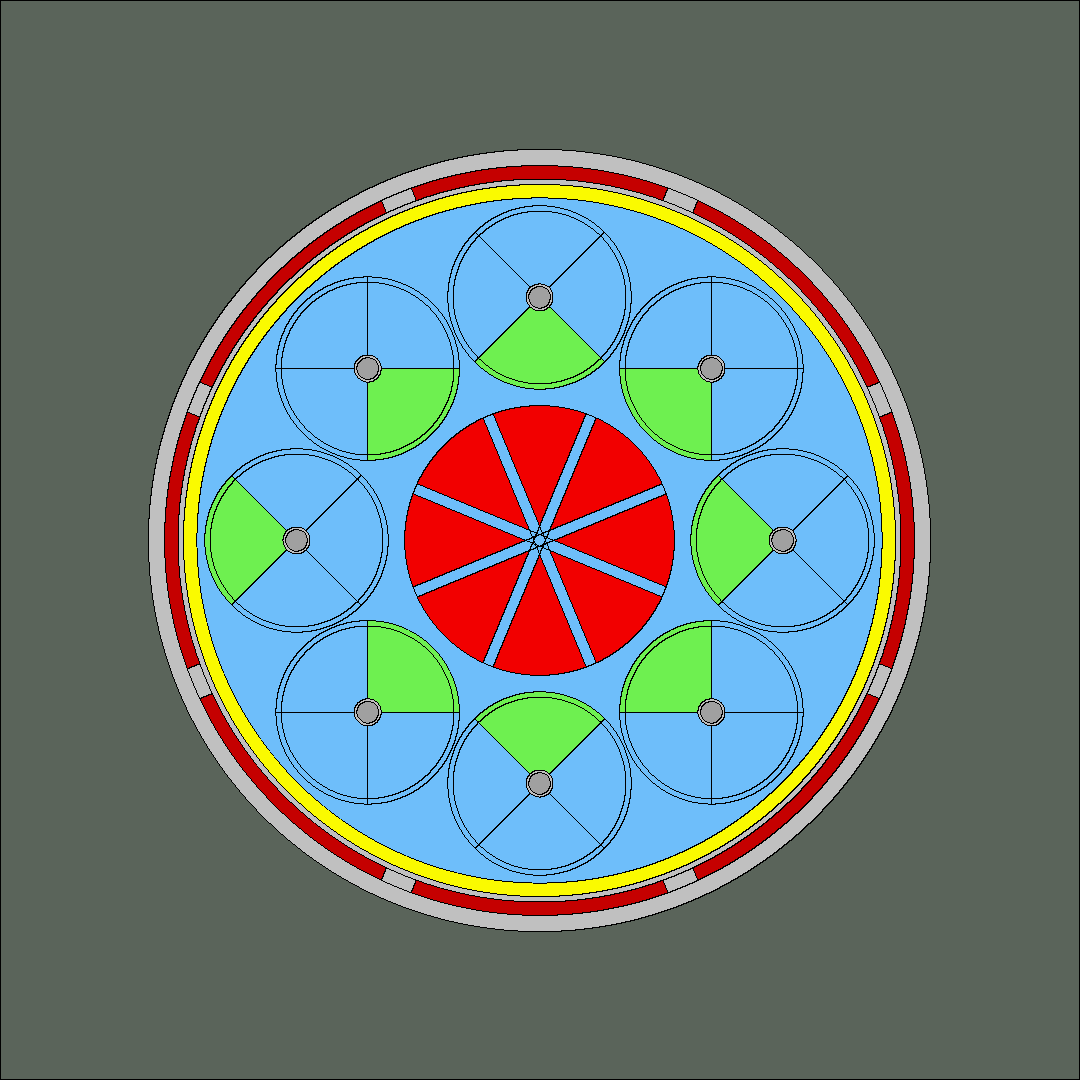
\includegraphics[width=0.49\textwidth]{Plotter/0.0shutdown7drum/MSNB_geom4}}
    \subfloat[\centering Single Success]{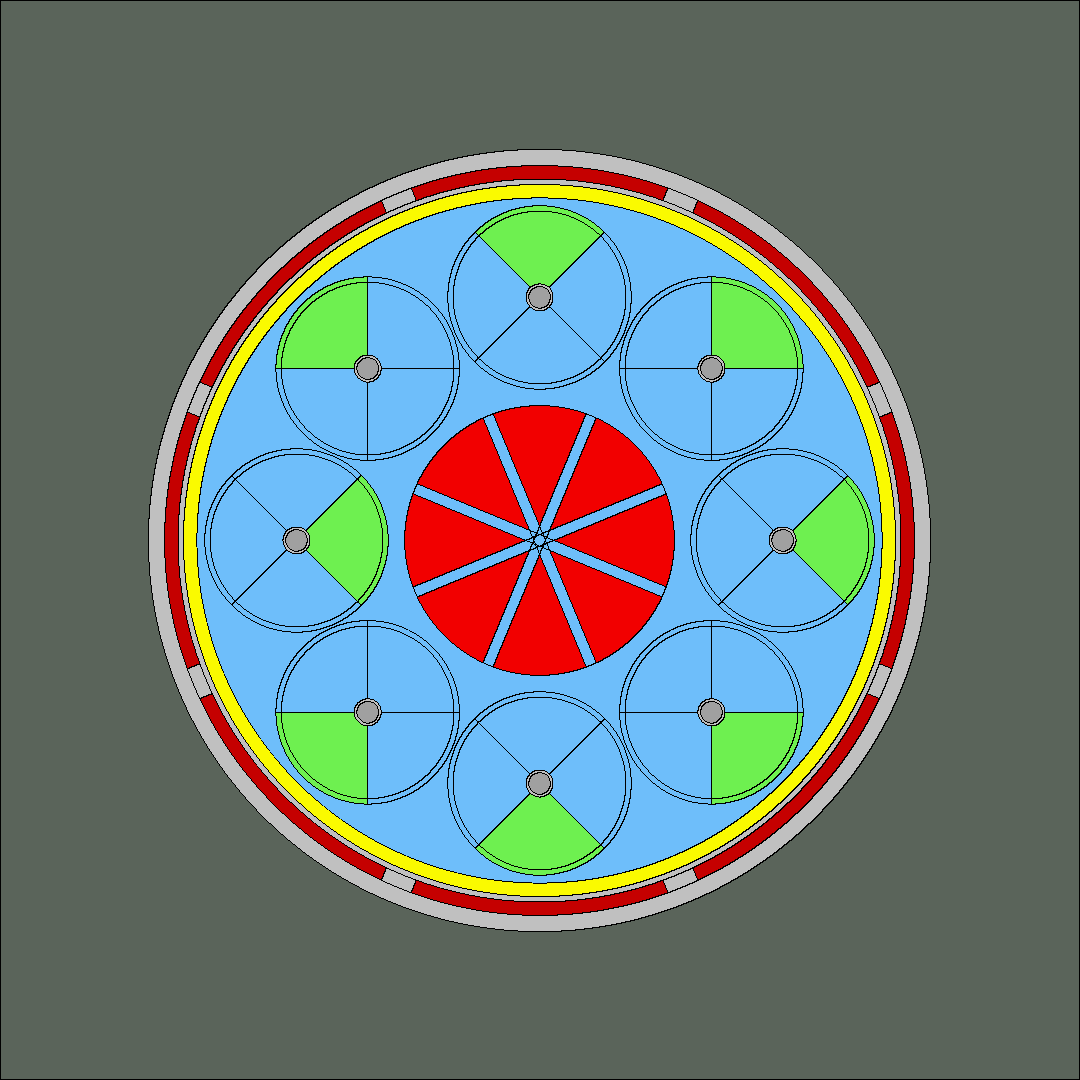
\includegraphics[width=0.49\textwidth]{Plotter/0.0shutdown1drum/MSNB_geom4}}
    \caption[X-Y View of \acs{msnb} - Shut-Down Margin]{X-Y Views of \acs{msnb} with control drums in two shut-down margin failure modes:
    \begin{enumerate*}[label=\alph*)]
        \item Seven drums in least reactive orientation, one drum failed in most reactive orientation; and 
        \item One drum in least reactive orientation, seven drums failed in most reactive orientation; 
    \end{enumerate*}
    }
    \label{fig:Plotter-SDM}
\end{figure}




including burned B4C

\subsection{Neutron Spectra}
\begin{figure}[ht!]
    \centering
    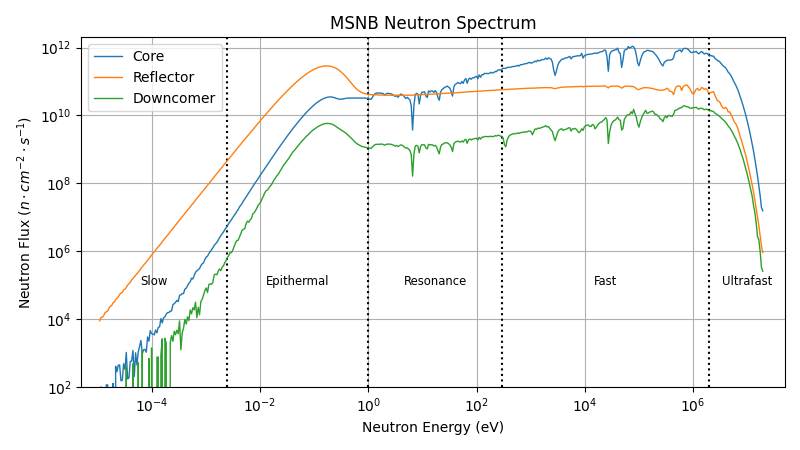
\includegraphics[width=0.9\textwidth]{./Plotter/Detector/Spectrum}
    \caption[\acs{msnb} Neutron Energy Spectrum]{\raggedright \acs{msnb} neutron energy spectrum in core, reflector, and downcomer.}
    \label{fig:Spectrum}
\end{figure}


\subsection{Actuator Curve}\label{sec:actuator}

\section{Multi-physics Simulation}

\subsection{Steady-State}

\subsection{Up-Step}
autonomous
controller tuning
controlled response


\subsection{Down-Step}

\subsection{Start-Up}

\subsection{Shut-Down}

\subsection{Demand-Response}

% -- Final Remarks --
\chapter{Conclusions}
\label{Chapter:Conclusions}

\section{Limitations}


\section{Future Work}\label{Chapter:Conclusions-FutureWork}
\subsection{Fuel Salt Thawing}
Because microreactors are meant to be delivered in a fully or mostly assembled state, it is likely that the \acs{msnb} will be shipped with the molten fuel/coolant salt mixture frozen \textit{in-situ}. The salt will need to be melted before initial start-up, and the heat source for melting the cannot be fission, as the \acs{msnb} requires advective heat removal caused by natural circulation; this is not possible if the flow channels between the core and heat exchanger are frozen. One possible method for salt thawing involves passing low-voltage high-current electricity through the pipes in contact with the salt, similar to how frozen water pipes are thawed \cite{Thawing}; this would be coupled with the introduction of hot secondary coolant into the heat exchanger to provide the necessary hot reservoir.

\subsection{Neutron Source}
A neutron source will be required to start the fission chain reaction after installation, and after any long periods of inactivity. \U[235] undergoes spontaneous fission \cite[Ch. 6]{Faw}, and at high enrichment may be used as the only neutron seed simply by putting the control actuators in a supercritical orientation. More commonly, a dedicated source is used, such as \Ca[252], which undergoes spontaneous fission much more rapidly, or a composite of a strong alpha-emitter (\eg \Pu[238], \Am[241], \Po[210], or \Ra[226]) and \Be[9] which emits a neutron according to \ref{rxn:Be-n} \cite[Ch. 2]{Handbook}. Dedicated neutron seed materials composed of these nuclides could be placed in the core through specialized mechanisms, though the introduction of the seed species as a soluble salt warrants a feasibility analysis.  

\begin{reaction}\label{rxn:Be-n}
    ^{9}Be + \alpha \to {^{12}C} + n + \gamma
\end{reaction}

\subsection{SCRAM System}
The emergency shutdown (\ie SCRAM) system must be passive. In \acsp{lwr}, this is achieved by including large control rods which are actively held out of the core, so that a loss of power results in automatic insertion. Larger \acs{msr} designs may include a SCRAM tank into which the fuel/coolant salt drains in the event of power failure. These systems are often actuated by a freeze plug \cite{FreezePlug} and put the salt in a subcritical orientation by the inclusion of neutron control materials \cite[Ch. 1]{Charit} and high geometric buckling \cite[Ch. 6]{Lamarsh}.

In the \acs{msnb}, the control drums will be actively actuated such that loss of power results in a negative control reactivity insertion of the greatest possible magnitude. Still, a freeze plug SCRAM tank system should also be included to make the system truly fail-safe \note{how to emphasize that this is author opinion}

\subsection{Decay Heat Removal}
Thermal power continues to be released by the decay of radio-nuclides after the fission chain reaction is stopped. For non-emergency shut-down, this heat may be removed by the same heat exchanger used for the secondary loop. There should also be a passive system that rejects decay heat in the event of total power failure, such as a direct contact system which removes heat through the vaporization of sodium \cite{DecayHeat} in the scram tank. This latent heat driven system is ideal because it minimizes the possibility of the salt freezing due to over-cooling.

\subsection{Flow Rate Control}


\section{Summary Remarks}

% ------------------------------------------------------------
% -- References -- 

\clearpage
\renewcommand\bibname{References}
\addcontentsline{toc}{chapter}{\bibname}
\bibliographystyle{nsf}
\bibliography{References.bib}

% ------------------------------------------------------------
% -- Appendices --
\clearpage 
\appendix % Marks start of appendices

%Test
%\chapter{Test}


\begin{code}\caption{Hello!} \begin{python}
    print("Hello World") #comment
    try:
        a=2/x
    except ZeroDivisionError:
        print('undefined')
\end{python}\label{code:hello}\end{code}

Inline codes like \pyth{import numpy}

\begin{code}\caption{F strings}
\inputpython{py/test.py}{1}{3}
\label{code:fstrings}\end{code}
\chapter{Deck Writing Script}

\begin{code}\caption{drum.py}
    \inputpython{py/drum.py}{1}{11}
    \label{code:drum}\end{code}

\begin{code}\caption{salt.py}
    \inputpython{py/salt.py}{1}{22}
    \label{code:salt}\end{code}

\begin{code}\caption{makedeck.py}
    \inputpython{py/makedeck.py}{1}{43}
    \label{code:makedeck}\end{code}

\begin{code}\caption{cell.txt}
    \inputserpent{py/cards/cell.txt}{1}{44}
    \label{card:cell}\end{code}
    \clearpage
    \inputserpent{py/cards/cell.txt}{45}{91}
    \clearpage
    \inputserpent{py/cards/cell.txt}{92}{109}

\begin{code}\caption{surface.txt}
    \inputserpent{py/cards/surface.txt}{1}{25}
    \label{card:surface}\end{code}
    \clearpage
    \inputserpent{py/cards/surface.txt}{26}{67}
    \clearpage
    \inputserpent{py/cards/surface.txt}{68}{92}

\begin{code}\caption{drum.txt}
    \inputserpent{py/cards/drum.txt}{1}{25}
    \label{card:drum}\end{code}

\begin{code}\caption{salt.txt}
    \inputserpent{py/cards/salt.txt}{1}{48}
    \label{card:salt}\end{code}
    \clearpage
    \inputserpent{py/cards/salt.txt}{49}{94}

\begin{code}\caption{material.txt}
    \inputserpent{py/cards/material.txt}{1}{47}
    \label{card:material}\end{code}
    \clearpage
    \inputserpent{py/cards/material.txt}{48}{85}

\begin{code}\caption{physics.txt}
    \inputserpent{py/cards/physics.txt}{1}{14}
    \label{card:physics}\end{code}

\begin{code}\caption{plot.txt}
    \inputserpent{py/cards/plot.txt}{1}{10}
    \label{card:plot}\end{code}

\end{document}

% ** DO NOT PUT ANYTHING AFTER THE END OF THE DOCUMENT! **
